\documentclass[a4paper,titlepage]{scrbook}
\usepackage[toc,page]{appendix}

% encoding
\usepackage[utf8]{inputenc}

% look
\usepackage{scrlayer-scrpage}

% for own column layouts
\usepackage{array}

% graphics
\usepackage{graphicx}
\usepackage[labelfont=bf, font=bf]{caption}
\usepackage{subfig}
% colors
\usepackage[usenames,dvipsnames]{color}
% test solid conics
\usepackage{pst-solides3d}
% math symbols
\usepackage{amssymb, amsmath, amsfonts}
\usepackage{textcomp, gensymb,mathtools}
\usepackage{siunitx}
\usepackage{listings}
%\usepackage{txfonts,pxfonts}


%math theorems
\usepackage{pdfpages}
\usepackage{makecell}
\usepackage[]{algorithm2e}
\usepackage{amsthm}
\usepackage{enumitem}
\newtheorem{theorem}{Theorem}[section]
% tables
\usepackage{multirow}

\usepackage[
  pdftex,colorlinks=false,
  hypertexnames=false,pdfstartview=FitH,
  linkcolor=black,citecolor=black,
  urlcolor=black,pdfborder={0 0 0}
]{hyperref}
\usepackage{bookmark}

% own marginpar
\let\oldmarginpar\marginpar
\renewcommand\marginpar[1]{\oldmarginpar{\tiny #1}}

\DeclareFontFamily{OT1}{pzc}{}
\DeclareFontShape{OT1}{pzc}{m}{it}{<-> s * [1.10] pzcmi7t}{}
\DeclareMathAlphabet{\mathpzc}{OT1}{pzc}{m}{it}

\title{TitleYetToDecide}
\subtitle{}
\author{Subin Joseph\\392292}
\subject{Master Thesis}
%\date{January 2, 2013}


% tikz
\usepackage{pgf,tikz}
\usepackage{mathrsfs}
\usetikzlibrary{arrows}


\begin{document}

% titlepage
\thispagestyle{empty}
\enlargethispage{1cm}
\begin{center}
\vfill
{\large Master Thesis}\par
\vfill
\parbox{0.9\textwidth}{
\begin{center}
 \sffamily\bfseries\Huge
 Network Forensic System for Internet Scanners\end{center}
}
\vfill
by\par
\vspace{0.9cm}
{\large Subin Joseph P}\par
392292\par
\vfill
\today\par
\vfill

\includegraphics[width=0.3\textwidth]{images/TU_logo}\par
\vfill
University of Kaiserslautern\par
Department of Computer Science\par
Distributed Computer Systems Lab\par
\vfill
\begin{tabular}{rl}
 First Examiner:  & Prof. Dr.-Ing. Jens B. Schmitt\\
 Supervisor: & M.Sc. Carolina Nogueira 
\end{tabular}
\end{center}


\chapter*{Abstract}
\thispagestyle{empty}
As the Internet technology advances and number of connected nodes on the Internet
become very high, network security has turned out to be  one of the most important factors for organizations to consider.
Port scanning is one of the networking tools attackers use to understand the vulnerabilities in the network.
It is a robust technique used to discover the services running on a target machine.
While port scanners can be used for many research purposes, there is a high chance
of mistreating their high potential by attackers to enumerate the vulnerable ports in the
Internet. 
So, it is important to do a systematic study on how these scanners behave by analysing the incoming connection requests from them.\\\\
Aiming at Internet scanner's detection, we develop a network telescope to capture packets.
Network telescope is able to provide a sampled view of the Internet with regard to
illegitimate traffic.
It accomplishes this by monitoring ranges of unused internet address space where no active services or servers reside. 
Our objective is to check whether it is possible to identify the internet scanners and get meaningful data about behavior of these scanners using the small network telescope. 
Packet capturing take place during two different schedules.
We initially use passive network telescope to capture the packets.
Here ports are closed and rejecting any incoming connection requests.
Since network telescope consists of limited IP address space, we latter combine the initial system with honeypot to exploit the received connections by sending vulnerable replies.\\\\
This thesis focuses on the analysis, manipulation and visualisation of the packets captured from the two above mentioned setups and check if it is feasible to identify a pattern depending on the behavior of port scanners and transport layer protocols used to send the packets.
Moreover, it is also important to compare the obtained results of the initial configuration with the latter structure and check if the behavior has been changed.
Analysis was achieved by selecting correct suitable metrics that were used
to extract information from captured traffic. 
Through correct visualisation, we could infer the relevant information from obtained results of the analysis for further research. 

 
\chapter*{Zusammenfassung}	
\thispagestyle{empty}
Da die Internet Technologie-Fortschritte und die Anzahl der verbundenen Knoten im Internet sehr hoch werden, hat sich die Netzwerksicherheit als einer der wichtigsten Faktoren für die Unternehmen erwiesen.
Port-Scannen ist eines der Netzwerk-Tools Angreifer verwenden, um die Schwachstellen im Netzwerk zu verstehen. 
Port-Scanning ist eine robuste Technik, die verwendet wird, um die auf einem Zielcomputer ausgeführten Dienste zu entdecken.
Obwohl Port-Scanner für viele Forschungszwecke verwendet werden können, gibt es eine hohe Chance, ihr hohes Potential von Angreifern zu misshandeln, um die anfälligen Ports im Internet aufzuzählen. 
So ist es wichtig, eine systematische Studie darüber zu machen, wie sich diese Scanner verhalten, indem sie die eingehenden Verbindungsanfragen von ihnen analysieren.\\\\
Netzwerk-Teleskop ist in der Lage, eine abgetastete Sicht auf das Internet in Bezug aufIllegitimer Verkehr.
Es führt dies durch die Überwachung von Bereichen von unbenutzten Internet-Adressraum, wo keine aktiven Dienste oder Server wohnen.
Unser Ziel ist es zu prüfen, ob es möglich ist, die Internet-Scanner zu identifizieren und mit dem kleinen Netzwerk-Teleskop sinnvolle Daten über das Verhalten dieser Scanner zu erhalten.
Die Paketaufnahme findet während zwei verschiedenen Zeitplänen statt.
Wir verwenden zunächst passives Netz-Teleskop, um die Pakete zu erfassen.
Hier werden Ports geschlossen und alle eingehenden Verbindungsanfragen abgelehnt.
Da das Netzwerk-Teleskop aus begrenztem IP-Adressraum besteht, kombinieren wir letztere das ursprüngliche System mit Honeypot, um die empfangenen Verbindungen durch das Senden von anfälligen Antworten zu nutzen.\\\\
Diese Arbeit konzentriert sich auf die Analyse, Manipulation und Visualisierung der aus den beiden oben genannten Setups aufgenommenen Pakete und prüft, ob es möglich ist, ein Muster zu identifizieren, abhängig vom Verhalten von Port-Scannern und Transportschicht -Protokollen, die zum Senden der Pakete verwendet werden.
Darüber hinaus ist es auch wichtig, die erhaltenen Ergebnisse der Anfangskonfiguration mit der letzteren Struktur zu vergleichen und zu überprüfen, ob das Verhalten geändert wurde.
Die Analyse wurde durch die Auswahl korrekter geeigneter Metriken erreicht, die verwendet wurden, um Informationen aus dem erfassten Verkehr zu extrahieren.
Durch eine korrekte Visualisierung konnten wir die relevanten Informationen aus den Ergebnissen der Analyse zur weiteren Forschung ableiten.
\chapter*{Eidesstattliche Erkl\"{a}rung}
\thispagestyle{empty}
Ich versichere hiermit, dass ich die vorliegende Masterarbeit mit dem Thema ``Network Forensic System for Internet Scanners'' selbstst\"{a}ndig verfasst und keine anderen als die angegebenen Hilfsmittel benutzt habe. Die Stellen, die anderen Werken dem Wortlaut oder dem Sinn nach entnommen wurden, habe ich durch die Angabe der Quelle, auch der benutzten Sekund\"{a}rliteratur, als Entlehnung kenntlich gemacht.

\vspace{3cm}
\noindent
\begin{tabular}{p{0.45\textwidth}p{0.45\textwidth}}
 \rule{0.4\textwidth}{1pt} & \rule{0.4\textwidth}{1pt}\\
Kaiserslautern, 31-July-2017 & Subin Joseph Poothiyottuthottathil
\end{tabular}




%\chapter*{Declaration of Academic Honesty}
%Hereby I declare that the present thesis is drawn up after MPO Elektrotechnik und Informationstechnik by myself without help of third parties but the support of my supervisor, that all used sources and tools including the internet are completely and exactly mentioned, and that everything is marked which is taken unchanged, shortened or analogous from other literature.
%
%\vspace{3cm}
%\noindent
%\begin{tabular}{p{0.45\textwidth}p{0.45\textwidth}}
% \rule{0.4\textwidth}{1pt} & \rule{0.4\textwidth}{1pt}\\
% Place, Date & Carolina Pereira Nogueira
%\end{tabular}

\newpage

\pagenumbering{Roman}
\setcounter{page}{0}
\tableofcontents
\clearpage

\setcounter{page}{0}
\pagenumbering{arabic}


\chapter{Introduction}
Computer networks and systems have turned out to be vital instruments for current business.
The amount of data that is stored and accessed by users throughout the world have been increased tremendously during last one decade.
According to Cisco's Visual Networking Index initiative \cite{cisco}, it is estimated that, before the end of 2016, worldwide Internet traffic will achieve 1.1 zettabytes per year and by 2019, global traffic is anticipated to hit 2 zettabytes for every year.
Much of this information is to some degree confidential and its protection is required.
As the number of connected nodes on the Internet has been increased, the various malicious attempts to gain control of the network is also increased.
Attackers use different networking tools like IP spoofing and Internet wide scanning to understand the vulnerabilities in the network.
So it is essential to build network security monitor devices to help uncover attempts by attackers to gain unauthorized access to computer networks.
This results to gain easy access to data stored in devices\\\\
Internet wide scanning is a robust technique used by researchers to study and evaluate Internet.
It has become popular in research field to learn new types of vulnerabilities, to track many risk mitigation activities.
However such a powerful tool could be used by attackers to locate  opened/vulnerable ports.
So it is important to do a systematic study on how these scanners behave by analysing the incoming connection requests from them.
This can be achieved using a Network telescope \cite{caida} which captures received packets and analyse it.\\\\
Network telescopes (NT) permit the capture of illegitimate data on a wider scale.
In general, NT captures the incoming traffic from an unutilised or dark Internet address space.
Network telescope is capable of detecting large scale of events with respect to the address spaces it monitors.
If an NT is being assigned with more Internet address spaces, its resolution will be also high \cite{irvin}.


% 	\section{Research Question}
% 		%  1. a concise statement of the question that your thesis tackles 
% 		%  2. justification, by direct reference to section 3 that your question is previously unanswered
% 		%  3. discussion of why it is worthwhile to answer this question.
	
	\section{Problem Statement}
	The volume of backscatter or Internet Background Radiation (IBR) \cite{pang2004characteristics}\cite{wustrow2010internet} has been increased excessively with the growth of Internet after its commercialisation in mid 1990s.
	Despite of the fact that, this is partly due to the system misconfiguration, a significant portion of such traffic can be seen as the result of either deliberate attack or network scanning tools.
	Moreover there has been an increase in spreading of malicious software or malware during recent years.
	Thereby the volumes and intensity of what is deemed to be traffic with malicious intent arriving at the Internet hosts are also increased.\\\\
	While Internet scanners can be used for many research purposes, there is a high chance of mistreating their high potential by attackers to enumerate the vulnerable ports in the Internet.
	The aftermath of all these attacks is that systems and organisations exposed to the Internet are facing a greater level of risk than they had before.\\\\
	Aiming at Internet scanner's detection, we developed a small network telescope. 
    Packet capture took place during two different schedules.
    We initially used active network telescope to capture the packets assuming that all the packets received by the network telescope are illegitimate packets.
    The active network telescope is called so since it is capable of receiving the incoming traffic and just responds to it.
    However, our configuration was designed in such a way that only port 22 was open and able to respond to the connection requests for accessing the dataset through SSH service.
    The remaining ports were closed during the first stage and rejecting any incoming connection requests.
	Since proposed system consists of limited IP address space, we later combined the initial system with honeypot to exploit the received connections by sending vulnerable replies.
	The honeypot was setup in such a way that it responds and process the requests to entire TCP network range and some UDP services with a legitimate service-like behavior.
	The main goal of the thesis is to analyse the received packets from the two previously mentioned setups and check if it is feasible to identify a pattern depending on the behavior of these scanners and transport layer protocols used to send the packets.
	Moreover it is also important to compare the obtained results of the initial configuration with the latter structure and check if the behavior has been changed.
	
    
	
\chapter{Background and Terminology}
Network telescope is responsible for capturing data from nefarious and potentially malicious traffic found on the internet.
The obtained dataset is analysed by making use of set of specific rules and utilize them to gather necessary information.
This information has to be made use of in an efficient manner.
By plotting the diagrams, one can decipher and comprehend what the information represents.
This thesis involves the gathering of such information, analysing and visualizing it by plotting the graphs.\\\\
One of the reasons for the anomalous unsolicited traffic are malicious network scans.
Scans are used to locate vulnerable computers in the network by automated or manual attempts from the user.
Internet threat monitors continuously observe many types of scans including methodical scans targeting single or multiple ports successively through an IP address range, continuous scans of ports on a single IP address and even ping based scans to check whether the device is existing on a given IP address.\\\\
This chapter will discuss the concept of network telescope, internet scanner (port scanner), honeypots and other related concepts which will be essential for the better understanding of rest of the paper.
    \section{TCP 3-way Handshake Process}
    Before discussing about Internet scanner and different types of port scanning methods, it is desire to have a basic knowledge about how TCP setup a TCP/IP connection over an Internet Protocol based network.
    TCP is one of the important protocols of the TCP/IP suite.
    It is connection oriented protocol as it provides reliable, error free, ordered communication between two hosts in a network.
    In order to provide the features mentioned above to the applications, it setup communication between the two devices that wish to communicate.
    This procedure typically called connection establishment, includes a trade of messages that moves both devices from their initial connection state (CLOSED) to the normal operating state (ESTABLISHED) \cite{rfc761}.
    \begin{figure}[t]
    \centering
	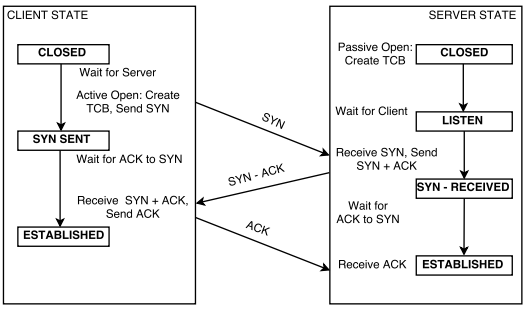
\includegraphics[width=10cm, height=6cm]{images/tcp_handshake.png}
	\caption{TCP 3-Way Connection Establishment Procedure}
	\end{figure}
	\\\\
	Figure 2.1 illustrates how the connection is established between two applications.
	TCP maintains data about each connection separately.
	This can be achieved by TCP with a special data structure called transmission control block (TCB).
	Before the process of setting up a TCP connection can begin, client and server create TCB to hold the information about it.
	To establish a connection between two devices, they should both send a SYN message and receive ACK for it.
	So the connection establishment involves three steps.
	Initially client sends a SYN message to the server. 
	Server sends the message that combines the ACK message for the client's SYN and SYN message for client.
	Finally client acknowledges the SYN message of server by sending an ACK to server.
	Thus connection is established between two devices.
	\section{Internet Scanner}
	Network scanning is a powerful tool utilized by analysts to study and measure the Internet and by attackers to enumerate vulnerable targets.
	There are two kinds of port scanning approaches existing nowadays: horizontal scanning which targets single port (process of scanning large number of hosts on a single port) and scans distributed across infected botnet hosts \cite{allman2007brief}\cite{dainotti2012analysis}\cite{czyz2013understanding}\cite{pang2004characteristics}.
	The idea of Internet scanners evolved during the late 90's by the initial release of NMap scanner \cite{lyon2009nmap}.
	After that many researches have been taken place in this field and many Internet scanners have been implemented.
	While well popular scanners like NMap provides many features like port scanning, host discovery, OS detection, it requires months to complete full scan over the Internet.
	However high speed Internet scanners like ZMap \cite{durumeric2013zmap} and Masscan \cite{graham2014masscan} take only few minutes to scan the entire IPv4 address space\\\\	
	As mentioned before, several Internet scanners are available such as ZMap, Masscan and NMap.
	Each of these scanners shows different characteristics based on their motives and how it is implemented.
	Since ZMap is currently one of the most well known Internet scanners, we choose it to explain the general working methodology of such scanners.
	ZMap \cite{durumeric2013zmap} is a high speed Internet-wide scanning tool which was developed by set of computer scientists from University of Michigan.
	One of the main advantages of ZMap is, it is able to complete a scan which targets at particular port or service of whole Internet from a dedicated computer in less than 60 minutes.
	It has one programming segment which sends the packets by using raw network sockets, thus cleverly avoids any overheads of the TCP stack.
	And another segment is used to gather and save any responses.
	Moreover ZMap allows to send more than 1 million probe packets at every second by bypassing the TCP stack, and a \SI{1}Gbit/sec outbound connections.
	\subsection{How ZMap differs from other scanners}
	In other network scanners like NMap, the Ethernet frame send by the users will be delivered to the target system much slower than high speed scanners, as well as the replies to source address.
	This is  due to the presence of network protocol overhead and inefficient method to avoid saturating the source or target networks.
	NMap scans the entire IP address range in numerical address sequence as well as it sends the packet to each IP address and waits for a reply.
	It also maintains state for each connection to keep track of previous scans and to deal with re-transmission and timeouts.
	As a result, there is a high probability of network congestion in the network being examined, thus resulting in a Denial of Service (DoS).\\\\
	ZMap tackled this issue by utilizing a technique called cyclic multiplicative groups.
	ZMap uses an iterative formula to visit every whole number from 1 to {$2^{32}$ – 1} (zero is omitted) at once, in a pseudo random order.
	So the probability of targeting single subnet at the same time during huge number of tests is lower.
	In view of this reason, ZMap does not make any part of the network busy or cluster the traffic in any part of the web.
	ZMap does not re-transmit the packets to avoid keeping the state, as it always sends a constant number of probes per target.
	Moreover ZMap is equipped for scanning the whole IPv4 addresses 1300 times quicker than Nmap's most proficient scanning setting.
	\subsection{How Internet scanners hide port scanning activity}
	Due to security concerns, organizations started deploying network security mechanisms such as firewalls to reduce the network activity.
	After the wide use of Internet scanners, people began adding the security features to firewalls to detect and block port scanning activity.\\\\
	Nevertheless, Internet scanners use variety of methods to obscure the port scanning activity, thus evade the detection of port scanning mechanisms. 
    For instance, Nmap provides its customers the ability to change the order of and timing between packets and randomize destination IPs \cite{lee2003detection}.
    It allows users to randomize each group of up to 16384 hosts before it scans them.
    This can make the scanning activity less evident to different network security systems, particularly when it combines with slow timing options \cite{nmap1}.\\\\
    Another way to avoid the detection is to use spoofed IP or IP decoys to conceal the attacker's IP address.
    Internet scanners enable users to use spoofed IPs to spoof the scan to make the targets believe that another person is scanning them.
    Furthermore, it permits to use IP decoys to perform decoy scan, which give a feeling to the remote target that the IP addresses you specify as decoys are scanning the target network as well \cite{nmap1}. 
    It results to make network monitoring systems behave like, it reports multiple scans from the same IP address. 
    Hence they cannot understand which IP was scanning them and which were innocent decoys.
    \subsection{Scanning Methods}
    Port scanning tools are widely used by attackers to identify the vulnerable ports and network administrators to study and correct the weakness in their own administrated network.
    Port scans often consider as the elementary step for attackers to find the vulnerable hosts or network and get access to it.
    Attackers use different scanning methods to scan the target hosts or network, to understand which service can be exploited to get the necessary information. 
    Port scan tools offer different scan techniques and users can choose the appropriate one according to their purpose.\\\\
    Selecting the appropriate scan methods is one of the most important decisions a user has to make while planning port scan attacks.
    Port scanning tool provides several port scanning techniques that gives the client the flexibility to create scans which might be more appropriate than using other techniques.
    Different types of port scanning techniques are listed below.\\\\
    \textbf{TCP SYN scan} -  SYN scan is relative simple and quick scan and can scan a large number of ports in every  seconds. 
    Figure 2.2 shows the process of TCP SYN scan  of an open port on the left, and of a closed port on the right.
    \begin{figure}[t]
    \centering
	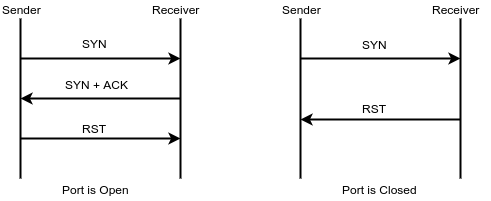
\includegraphics[width=10cm, height=6cm]{images/tcp_synscan.png}
	\caption{TCP SYN Scan Process}
	\end{figure}
    It  works  in  such  a  way  that  it  does not  finish  the  3-way  TCP  handshake mechanism.  
    It  just  sends  an  initial  SYN  signal  and  wait  for  the  SYN-ACK  message from  the  target.
    If the sender receives the SYN-ACK message, it sends RST message to the target and connection is not established.
    However, if the port is closed, target system sends RST message to the sender.
    Since it does not establish the connection, it is also known as TCP half open scan.\\\\
    \textbf{TCP Connect scan} -  TCP  connect  scan  is resource sensitive and slower scan compared to TCP half open scan.  It completes the handshake mechanism and establish a connection by sending the ACK packet, but close the connection just after it.
    As the target system assign resources to enable the TCP connections during TCP connect scan, it can cause performance issues on the target system.
    In addition to that, this sort of scan is easily detectable and filterable.\\\\
    \textbf{TCP NULL, XMAS, FIN scan} - Another approach to utilize the TCP protocol to gain information about the target system are TCP Null, Xmas, FIN scan. 
    These scanning methods are known as stealth scans, as TCP header flags are setup in such a way that it will gain necessary information back from target system without attempting for connection establishment or establishing the connection.
    It differs from the TCP SYN and connect scan as it attempts to collect the information during  TCP three way handshake process.
    While TCP Null, FIN and Xmas scans analyze the packets, which
    follow to the corresponding packets sent from the scanner to the scans victim.\\\\
    The null scan does not set any bits and its TCP header flag will be empty.
    If the port is open, these packets will be ignored by the target system as these packets are invalid and would never occur in the real world.
    However, if the port is closed, sender receives a RST packet as the port is unreachable.\\\\
    The FIN scan sends the packet by just setting the FIN flag in the TCP header to the target system.
    This kind of TCP packets are generally used to terminate an established connection.
    If the port in the target system is closed and it receives the FIN packet without establishing a connection with sender, it reacts with a RST packet.
    If sender does not receive any response from host system, the port is considered open.\\\\
    During Xmas scan the port scanner sends TCP packets in which FIN, PSH (PUSH) and URG (Urgent) flags in the TCP header are set \cite{port_techniques}.
    The URG flag is used to inform a receiving station that certain data within a segment is urgent and should be prioritized.
    The PSH flag in the TCP header informs the receiving host that the data should be pushed up to the receiving application immediately.
    If the sender does not receive any response to the packet from the target system, the port is considered open and if a RST packet is received, the port is considered closed.\\\\
    \textbf{UDP scans} - UDP port scans are another type of port scanning activity which is based on UDP protocol.
    Since UDP is a connection-less protocol, UDP scanning is generally slower and difficult to implement than TCP.
    UDP scan works by sending an UDP packet to every targeted port.
    If the destination port is closed, the system will respond with ICMP port unreachable error (type 3, code 3) message.
    If no response is received after sending the packet, the port is considered as open.
    It generally re-transmit the packets to ensure that packet is not lost while transmission thereby reaffirm port is open.
    However, if port is filtered by a firewall, this method will falsely report that port is open \cite{de1999review}.\\\\
    Another approach is to send packet with protocol-specific payload to some common destination ports to increase response rate.
    This method is much more reliable at identifying open ports.
    However, it is limited to scanning some common ports for which an application probe packet is available.
    Some port scanners such as nmap generally have probes for less than 20 UDP services, while some commercial tools (e.g., nessus) have as many as 70. In some cases, a service may be listening on the port, but configured not to respond to the particular probe packet \cite{port_techniques}. 
	\section{Network Telescope}
	The idea of Network Telescopes as a method for monitoring activity on the Internet everywhere, has grown progressively since mid 2000.
	Network Telescope is a tool that monitors traffic destined to what is known as "Internet dark address space".
	These addresses are portion of routed, allocated IP address space in which no active services or servers reside.
	Since no legitimate packets travel through these address spaces, one can obtain information about possible network attacks as well as misconfigurations by watching the network traffic addressed to these IP addresses.
	Network Telescope  mostly carries  illegitimate traffic such as continuous view of anomalous unsolicited traffic, or Internet Background Radiation (IBR).
	IBR emerges from an extensive variety of events, such as backscatter resulted from spoofing, misconfigurations, scanning of IP address space by attackers or malware looking for vulnerable targets, and Internet worms.\\\\
	Traffic originating from Internet hosts and are received by network telescope can be classified as one of the following three broad categories:
	\begin{itemize}
	\item Backscatter - The traffic resulting because of the victims response to the spoofed packets as normally it would respond to the legitimate requests.
	This traffic comprises fundamentally of specific classes of ICMP traffic and of TCP packets with RST (reset) or SYN (synchronise) and ACK (acknowledgement) flags set.
	\item Configuration Mistakes - A traffic flow which occur due to the misconfiguration of the computers in the Internet. 
	This flow lives only for a short period of time.
	\item Host/Port scanning - The traffic that can be grouped as being originated from different scanning agents like ZMAP, NMAP, Massscan etc.
	\end{itemize} 
    Network telescope can be categorized in to mainly two: active and passive network telescope.
    Passive network telescope is able to capture the incoming packets, however is unable to respond to these packets.
    Active network telescope responds to the incoming packets and try to establish the connection using 3-way TCP handshake.
    \subsubsection{Passive Network Telescope}
    Passive network telescope observes the network traffic targeting the address space of the network but is insufficient to respond to any of the incoming packets.
    It is unable to complete the 3-way TCP handshake which is the requirement for starting the actual transmission of TCP data.
    However it is able to receive the payload data from UDP and ICMP packets as they are connection less protocols.
    \subsubsection{Active Network Telescope}
    Active network telescope is able to respond to the incoming connection requests captured by it.
    It can respond to the 3-way TCP handshake mechanism thus able to receive the TCP payload from the remote connections.
    A responder replies to a TCP SYN request with a TCP SYN-ACK packet and in so doing receive the first packet containing a data payload \cite{bailey2006practical}.
    Thus actual data can be used to get a better understanding about the remote connections.
	\subsection{The Case for Monitoring}
	Nowadays, it is essential to find a solution to understand  and respond to rising dangers in the Internet.
	Data security specialists both in the scholarly community and at security sellers first need to be capable to isolate and study both the behaviours of the actual binary files associated, but also the behavioral perspectives related to the worldwide system-the Internet.
	The monitoring of network services can be categorised in to two main types:
	\begin{itemize}
	    \item Passive Monitoring - One of the greatest issues with conventional monitoring schemes is the issue of differentiating between legitimate and unexpected traffic.
	    The utilization of network telescopes to tackle the monitoring issues above, can in some ways alleviate these difficulties.
	    This can be accomplished, by observing just the activity that is not part of legitimate traffic,  and therefore already potentially suspect. 

	    \item Distributed Monitoring - The importance of monitoring the networks has been increased inspired the implementation of the distributed networking.
	    It consists of  multiple smaller sensors or alternately a single sensor with multiple smaller address allocations to monitor.
	    Distributed monitoring makes sense, if an organisation has larger address space, or sufficiently fortunate to have numerically non-contiguous address space.
	\end{itemize}
    There may be some security concerns within an organisation when a network telescope is established.
    Some of the potential threats to passive sensors are discussed in the \cite{shinoda2005vulnerabilities}.
    Considering this, an accurately configured framework ought to prove an advantage for an association's Information Security toolset, instead of a risk.
    \subsection{Analysis of Network Telescope Traffic}
    Packets received by the network telescope can be classified as internet worms, backscatter resulted from spoofing, misconfigurations, scanning of IP address space by attackers or malware looking for vulnerable targets.
    These packets should be analysed carefully to understand the motive behind each packet.
    However this can be identified easily by just understanding the traffic and how it is generated.
    \begin{table}[t!]
    \centering
    \begin{tabular}{ |p{6cm}|p{6cm}|  }
    \hline
    Packet sent & Response from destination\\
    \hline
    TCP SYN (open port)   & TCP SYN/ACK\\
    TCP SYN (closed port) & TCP RST\\
    TCP RST & no response\\
    TCP ACK    &  TCP RST\\
    TCP NULL & TCP RST (ACK)\\
    UDP packet (open port)& Protocol Dependent\\
    UDP packet (closed port)& ICMP Port Uncreachable\\
    ICMP Echo Request & ICMP Echo Reply\\
    ICMP TS Request & ICMP TS Reply\\
    \hline
    \end{tabular}
    \caption{Packet Requests and Responses \cite{moore2006inferring}}
    \end{table}
    \\\\
    Each type of attack uses different mechanism to achieve its goal. 
    For example, the motive behind the DoS attacks is to consume the resource of its target, that can be a host or a network.
    To achieve that, SYN Flood mechanism is used where several SYN packets are sent continuously.
    For each SYN packet received by the destination host, it has to process that packet by storing the information about the connection requests, thus consume the resources of the host.
    These mechanisms are mostly influenced by the way the packet is requested and its response.
    The Table 2.1 shows the common packet requests and their responses.
    \subsection{Internet Threat Monitor}
	Due to the significance and usefulness of network telescopes, numerous projects and collective efforts have been taken place to explore the field of network monitoring.
	CAIDA, the Cooperative Association for Internet Data Analysis \cite{caida} started one of the initial works in the field of network monitoring and they use network telescope which is huge, routed, but very sparsely populated address block. 
    DShield \cite{dshield} a community-based collaborative firewall log correlation system took an another approach that collects firewall logs from participating system administrators.
    Many such monitoring systems have been deployed around the world due to the success of these systems.
    These systems can be commonly referred to as Internet threat monitors.
    \begin{figure}[t]
    \centering
	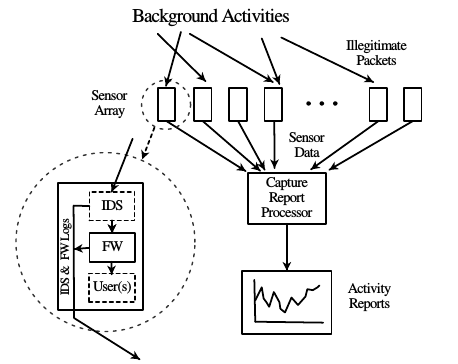
\includegraphics[width=8cm, height=6cm]{images/int_threat_mon}
	\caption{ Structure of a Typical Internet Threat Monitor \protect\cite{caida}}
	\end{figure}
	\\\\
	A typical Internet threat monitor can be seen in the Figure 2.3. 
	It comprises set of sensors listening to packets arriving at a set of IP addresses, capturing all traffic sent to these addresses.
	Sensors can be categorized in to passive and active based on the traffic it receives and how it responds to it.
	A passive sensor is configured to receive IBR traffic and no legitimate response is sent back to source.
	As such, it is difficult for a potential attacker or instance of malware to determine anything about the target system.
	Moreover since it does not reply to any incoming packets, it requires significantly less computing and bandwidth resources than active sensor.
	An active sensor replies to incoming IBR traffic to solicit further  traffic  so  as  to  more  precisely detect  its  nature  and intent.
	Examples include Internet motion sensor \cite{cooke2004internet} and honeypots.
	Server is the place where all data collected by the sensors is  stored, processed, analyzed and presented.
    \section{Honeypots}
    Honeypot is a computer security mechanism set to act as a decoy to attract malicious traffic.
    The main purpose of the honeypot is to detect, deflect and investigate the attempts to gain illegitimate access to information systems \cite{provos2004virtual}.
    It comprises a computer, applications, and information that reproduce the behavior of a genuine system that gives off an impression of being a piece of a system but is really detached and closely observed.\\\\
    Honeypots are similar in character to network telescopes.
    Both can be used to monitor the individual or range of IP addresses to capture the nefarious traffic.
    However the honeypot differs from network telescope regarding the method of capturing the  malicious packets.
    Honeypots actively communicate with a threat and attract the malicious traffic whereas network telescope just listens to the incoming traffic. 
    This enables honeypots to describe  the vulnerability that has been exploited and its effect on a machine \cite{bailey2005data}.\\\\
    Honeypots can be categorized in to mainly two based on its design criteria: low and high interaction honeypot.
    The low interaction honeypot emulates just services often requested by the 
    attackers, while a high interaction honeypot reproduces the behavior of a complete physical machine that host different services.
    By using honeypot, it is possible to learn more about the behavior of  different attacks such as how an attacker exploits the vulnerabilities in the system to  gain root access of the host.
    \section{Network Packet Analysing Tools}
    During the course of thesis, different packet analysing tools were used in order to analyse the capture files.
    It can be used to analyse the network traffic and generated customized report to assist researchers or organization in managing their networks.
    This section briefly explains the tools that were used during the thesis work.
    \subsection{Wireshark}
    Wireshark was developed in 1998 and is one of the widely used packet analyser in the world \cite{wireshark}.
    Wireshark provides a significantly more full highlighted graphical environment in which one can perform more useful analysis and filtering of the packets.
    It can be also used to dissect the part of the protocol and subsequently decoding the information for an encapsulated higher order protocols.
    Wireshark support libpcap file format (also known as pcap file format) which is popular file format for storing, reading and interchange of packet data.
    The biggest problem experienced with Wireshark is the inefficiency to load and work with files containing large number of packets.
    \subsection{Tshark}
    TShark is another version of Wireshark which is purely terminal based, works similar to tcpdump, but more powerful than it \cite{tshark}.
    It is used for capturing and filtering out packets when an interactive user interface is not accessible or required. 
    The two primary benefits of Tshark are that it can be used  on a remote computer through a SSH connection and as a part of scripts.
    
\chapter{Related Work}\label{chap:Background and Related Work}
    A large number of materials have been published relating to the applications and use of Network Telescopes as research tools.
    NT have been used for different research purposes including malware characterization, distributed denial of service, network scanning during previous years.
    This  chapter  addresses the recent researches in the field of internet scanning, network telescope and network traffic analysis.
    \section{Malware Characterization} 
    Network telescopes have been utilized effectively to portray malware distribution, and propagation.
    Most of the Internet worms spread by randomly generating an IP address as their destination address.
    Then it sends the worm to these IP addresses in the hope that it is used by some vulnerable computers.
    Since network telescope is routed, there is a probability that it also receives probes from hosts infected with worms.
    There by network telescope captures these infection attempts and analyses it.
    Conficker worm \cite{porras2009conficker} has been examined by the researchers by collecting data on network telescope in gaining better understanding about this worm \cite{irwin2012network}.
    The traffic produced by the Witty worm has been first examined by Shannon and Moore in 2004 \cite{shannon2004spread}.
    \section{Distributed Denial of Service (DDoS)}
    Network telescopes can be used to observe the distribute denial of service attacks.
    Attackers use fake IP addresses as the source IP address and send it to the victims.
    Since the victims are not able to distinguish between incoming requests from an attacker and legitimate inbound requests, it replies back to these source IP addresses considering it as legitimate connection requests.
    When the attacker uses the IP addresses in the network telescope IP address space for spoofing, NT can observe the response targeted for the computer that does not exit. 
    NT monitors these unsolicited responses and identify the denial of attack victims, and get the information about the types of applications the attacker targets, volume of attack, the location and bandwidth of the victims.
    The idea of monitoring background traffic started from CAIDA's network telescope in 2000 \cite{caida}.
    The backscatter datasets provided by CAIDA have been utilised for many legitimate research purpose as well as to understand the vulnerabilities of the network telescope.
    Many other notable  works have been published, which utilises network telescopes for understanding this type of traffic \cite{moore2006inferring}\cite{stavrou2005websos}\cite{kompella2004scalable}\cite{pouget2008understanding}.
    \section{Network Scanning }
    Network telescope have been applied in gaining better understanding about the traffic sent by the network scanners.
    The one of the first comprehensive works in this area have been conducted by Pang in 2004 \cite{pang2004characteristics}.
    It examines the most frequently scanned protocols in addition to different aspects of IBR.
    Wustrow et al. \cite{wustrow2010internet} provided a valuable insight in to Internet background radiation by updating the work done by Pang.
    They noticed a rise in scan traffic intended for well known ports such as telnet (TCP/23) and SSH (TCP/22).
    Furthermore an increased scanning activity reported on port 445 (SMB over IP) because of Conficker.\\\\
    The analysis by considerable amount of research works showed an increase in distributed botnet scanning during last decade \cite{leckie2002probabilistic}\cite{schechter2004fast}\cite{jung2004fast}.
    The recent study by Durumeric \cite{durumeric2014internet} implements a large network telescope to analyze the behavior of Internet scanning and identify the broad behavior of scanning activity.
    Moreover it shows a wide perspective of target protocols, the existing scanning methods, the intention of scanning, the source of scanning activity, and software they use for scanning.\\\\
    Several port scanning detection mechanisms have been developed during the previous years.
    However many of the past works relied up on a large network telescope consists of wide range of IP addresses.
    Moreover most of the previous works used passive network telescope which is  capable of receiving incoming traffic and has no means of responding to any packets.\\\\
    Our research basically varies from the previous works regarding the setting up of network telescope.
    Multiple factors need to be considered while configuring network telescope.
    The range of IP addresses assigned and category of network telescope are the two elements we considered while setting up the network telescope.
    Here we used considerably smaller network telescope which consists of 25 IP addresses and configured it both as active network telescope and network telescope with honeypot system during the data collection period.
    Our research work mainly focuses on the feasibility of port scanning detection from very small network telescope.
    Furthermore it analyses the received packets from the two separately configured network telescopes and check if the behavior is different in each configuration.
    
    
    
    
 
\chapter{Design}
The network forensics is the field of digital forensics in computer networks.
The objective is to monitor and anaylse the network traffic for the purpose of dealing with the network crimes.
Network forensics is defined as “the use of scientifically
proven techniques to collect, fuse, identify, examine, correlate, analyze, and document digital evidence from multiple, actively processing and transmitting digital sources for the purpose of uncovering facts related to the planned intent, or measured success of unauthorized activities meant to disrupt, corrupt, and or compromise system components as well as providing information to assist in response to or recovery from these activities” \cite{palmer2001road}.
The proposed network forensic system consists of a capture module, anaylsis module and visualization module.
The system is designed to capture the network traffic from the different hosts in the internet, categorize the port scanning packets, analyse it and visualise the needed information.
The capture module consists of a network telescope and a place to store the captured packets.
The purpose of the anaylsis module is to separate the port  scanning packets from other illegitimate packets.
The illegitimate packets can be denial-of-service attacks, Internet worms, malicious network scans or due to misconfiguration problems.\\\\ 
The suggested network forensics system which is designed to monitor the port scanning activities is shown in the Figure 4.1.
It consists of mainly three modules: capture module, analysis module and visualization module.
The capture module includes network telescope which is dedicated for capturing the IPv4 packets.
Each packet goes through the capture module and store it in hard disk.
The analysis module analyses each packet from the hard disk and decide whether it is port scanning packet or not. 
Afterwards it separates the port scanning packets from other illegitimate packets.
The visualization module uses the port scanning packets and provide the valuable information about the behavior of the port scanning.
\begin{figure}[t]
    \centering
	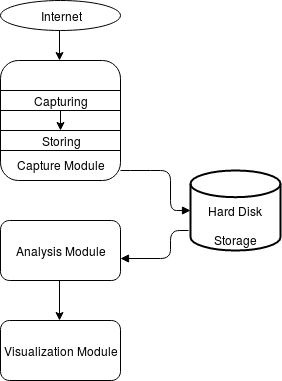
\includegraphics[width=7cm, height=8cm]{images/networkforensic_arch}
	\caption{ The Architecture of Network Forensic System}
\end{figure}
\section{Capture Module}
The primary task of the capture module is to capture the network 
activity that is capable of network attack.
This module can be subdivided into two sub modules: capturing and storing.
\subsection{Capturing}
\begin{figure}[t]
    \centering
	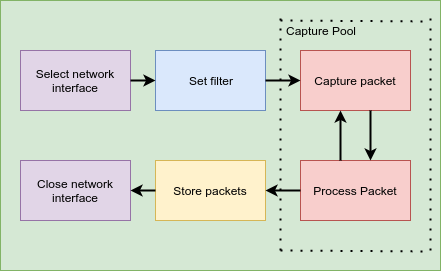
\includegraphics[width=10cm, height=6cm]{images/packetcapture_flow1.png}
	\caption{ Program Flow of Packet Capturing System}
\end{figure}
This module contains network telescope which capture all the incoming packets passing through the network interface of the host.
Network telescope is associated with packet capturing system, which actually does the work of collecting the packets that pass through a given network interface.
Packet capturing system is designed for UNIX system based on libpcap, an open source library that provides a high level interface to network packet capture systems.\\\\
Figure 4.2 shows the important steps in the  the packet capturing system.
Initially we need to select the network interface to listen on.
When the kernel gets a packet from the network interface, it has to copy the packet from kernel space to user space. 
Performing this task on every packet will reduce the performance of our packet capturing system and kernel may drop packets.
To counter this problem, we set a filter to avoid capturing packets from server address, thus capture packets only from  specific range of IP addresses.
After setting up a filter expression, we start capturing the packets and  dissect packet into different headers and process it.
These processed packets are stored in a separate file in the next step.
Once we decide to stop capturing process, we close the interface and exit from the capturing procedure.\\\\
The packet capturing process take place in two stages. 
In the first stage, the network telescope is designed as active in such a way that it does not send anything unless it receives a request. 
In the second stage, the network telescope is associated with T-Pot, a multi-honeypot platform system from Deutsche Telekom.
Network telescope configuration at these two phases will be explained in detail in Chapter 5.
\subsection{Storing}
Storage and processing are also significant aspects to consider, as traffic that has been captured needs to be stored somewhere for further analysis.
This module stores the captured packets to the hard disk of the host system, in order to do the further investigation on the packets.
Once the packets have been collected, storage provision needs to be made to store the packets.
Due to the limited size of the hard disk, we used the logrotate command to rotate the logfiles on weekly basis.
The UNIX logrotate utility can be used to rotate the log files when size of the file reaches a certain level.\\\\
These packets were stored in pcap file format which is a basic and common method to store captured network data.
We decided to store the packets in pcap format because of its immense popularity in network packet capture and exchange formats.
Pcap format is defined by libpcap, a portable C/C++ library for network traffic capture for UNIX systems.
Moreover popular networking tools such as tcpdump, Wireshark, libtrace, tcpsplice use pcap file format to capture and process the packets.
\section{Analysis Module}
\begin{figure}[t]
\centering
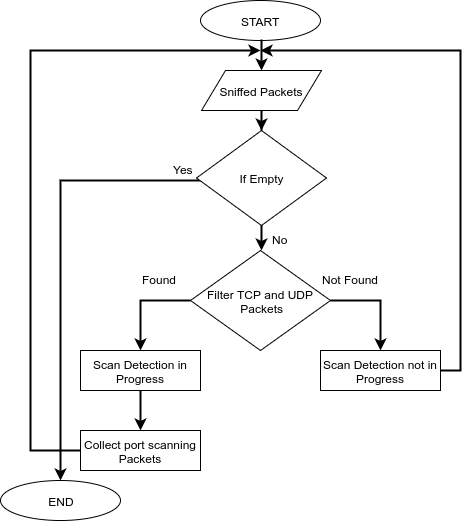
\includegraphics[width=8cm, height=10cm]{images/analysis_flow.png}
\caption{ The Data Flow Diagram of Port Scan Detection}
\end{figure}
The analysis module analyses the captured files stored in the system by the capture module, with a specific end goal to find the behavior and source of the  port scanning attack.
In order to do that, it is important to separate the port scanning packets from other malicious traffic.\\\\
The port scanning detection mechanism is basically designed  to detect TCP and UDP scans.
In addition to that, it divides port scanning activities into different categories.
The port scans can be divided into mainly two types based on the pattern of 
destination ports and target destinations the scan examines: vertical and horizontal scans.
The vertical scan is a port scan which targets multiple destination ports on a same IP address.
This is one among the easiest one to detect because only one host needs to be investigated. 
The horizontal scan is a port scan which scans multiple IP addresses, but targets only one specific port.
However Internet scanners provide several methods to hide the port scanning activity from the host system, thus avoiding the detection of port scanning mechanisms as explained in the Section 2.2.2.
One method to avoid the detection is to increase the timing between two successive scans in the same network or host.
In order to tackle this problem, we design our algorithm in such a way that it look for port scans from the same source for a definite amount of time. 
Another method to evade the detection is to scan from a block of addresses using spoofed IP or IP decoys.
We try to quantify this error using two methods.
Initially, we design an approach to minimize the false positives in the result by just combining the IPs from the same /24 network which target the same set of hosts and ports \cite{lee2003detection}.
The second method is a tentative approach to  minimize the error, by considering that possibly all attacks from same source come from the same Internet Service Provider (ISP).\\\\ 
Furthermore the port scanning activity can be divided based on the techniques users apply to scan the network.
The different techniques of the port scanning is explained in the Section 2.2.3.
We design our port scanning detection program to detect and categorize the incoming port scans into different scanning techniques.
Port scanning techniques we investigate include TCP SYN scan, TCP connect scan, UDP scan, Null scan and Xmas scan.
The port scanning detection mechanism and how the previously mentioned methods are implemented will be explained more in detail in next chapter.\\\\
The Figure 4.3 shows the data flow diagram of port scan detection.
After we capture the packets, we do the scanning detection activity on TCP as well as UDP packets and then collect port scanning packets.
We use these packets to do further investigation in the next stage.
\section{Visualization Module}
After the analysis of the packets, there should be a good mechanism to deduce the
relevant information for further research.
The visualization module provides simple and solid accessible way to plot the graphs, to gather more information about the behavior of port scanning.\\\\
The visualization module consists of several scripts to infer the valuable information by plotting the relevant graphs and numerical analysis.
The generation of graphical overviews of the data using these scripts is straightforward method in  understanding the data and trying to identify trends, and any particular areas of interest.
The graphical overviews serve to allow rapid high-level inspection of the data. 
Each script uses the results of the analysis module to display the information such as whether the port scanning attack was accomplished.\\\\
This module produces graphs such as correlation between the number of destination IPs and number of scans (horizontal scans), correlation between the number of destination ports and number of scans (vertical scans), relationship between traffic rate and the time of the day, geographical distribution of location of port scanning attacks etc.
These graphs will give a better perception about how attackers generally scan the network, what is the real purpose behind scanning activity, how frequently they do port scans etc.\\\\
We design the horizontal scan graph in such a way that, it gives a fair idea about how do attackers generally scan the network in the perspective of number of destination IPs targeted.
It uses a buffer to store the source IP address and corresponding targeted IP addresses for each port scan.
Vertical scans are essential when the attackers are interested in a specific destination IP address and they want to check if any of the services are available on the specific IP address.
So the vertical scan graph is designed to get a general behavioral pattern of the port scans based on the number of services targeted on a specific host IP address.
It also uses a buffer to store the source IP and corresponding targeted ports on a particular target system.
We are interested to learn the frequency of port scans of top 5 countries who participate in scanning activity based on the local time of the source of attack.
We consider the timezone of source of port scans to get the local time at which port scans executed.
So we propose a graph which shows the relationship between traffic rate and the time of the day for each country, to check if port scanning is a constant activity throughout the day or attackers are more interested in a particular time of the day to execute port scanning.
We also want to examine the location of port scans and which parts of the world are more involved in port scanning.
So a heat map is designed to show the geographical distribution of location of port scanning attacks.
Red color shows the location from which port scans take place most frequently, yellow color shows the location origin of less frequent port scans, and orange color displays the location that fits in between the condition of both yellow and red regions.
Furthermore information such as total number of packets
processed, total number of port scans, popularity of destination ports scanned are also displayed in this module.
\chapter{Implementation}
The suggested network forensic system is designed and implemented to detect and study the behavior of port scanning attack.
It is mainly divided in to three modules such as capture module, analysis module and virtualization module as mentioned in previous chapter.\\\\
The packet capturing system is used for capturing the packets and is installed in the network telescope.
It captures all kinds of the packets that pass through a given network interface and is implemented using C with libpcap library.
\begin{figure}[ht]
    \centering
	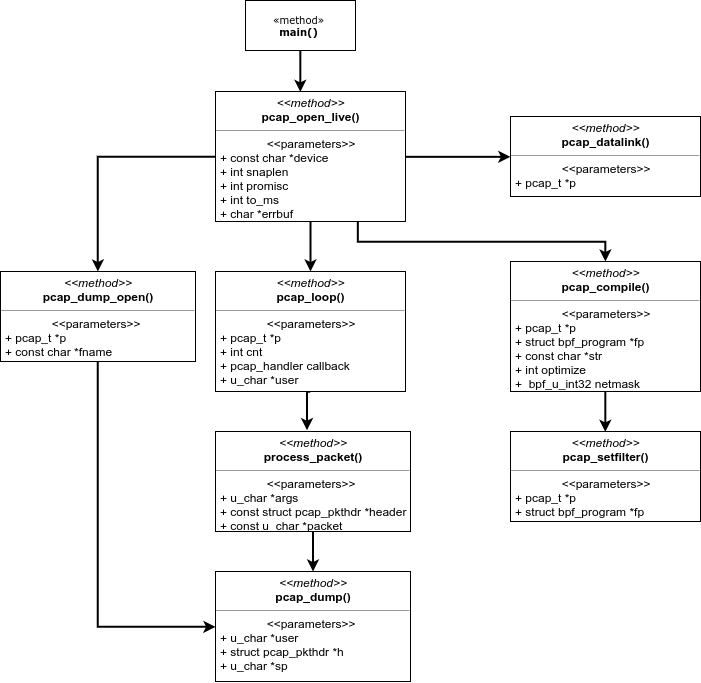
\includegraphics[width=10cm, height=12cm]{images/uml_packetcapture.png}
	\caption{Call Diagram of Packet Capturing System}
\end{figure}
\\\\
Figure 5.1 shows the important functions and how it is related to each other in packet capturing system.
We select the network device and open it using pcap\_openlive(), a function provided by libpcap library.
To capture all of the network traffic, we set up the network interface in to  promiscuous mode using promisc flag in pcap\_openlive.
This function returns an interface handler that will be used later when calling rest of the functions provided by libpcap.
Setting a filter involves three steps: constructing the filter expression, compiling the expression into a BSD Packet Filter (BSD) program and applying the filter.
We constructed the filter expression to remove the packets coming to server IP address from the captured dataset.
The expression is compiled using pcap\_compile() and inserted it into kernel calling the function pcap\_setfilter().
The pcap\_loop() is used to collect packets and process them.
This function calls a user defined function process\_packet() every time when there is a packet ready to read.
These packets are written to a capture file using the function pcap\_dump(). 
The captured files are stored in to hard disk and log files are rotated weekly using logrotate option in the UNIX.\\\\
The traffic collected by a network telescope provides a large dataset that needs to be analysed.
This can be achieved by a port scanning detection mechanism in the analysis module.
It is implemented separately in an another machine  which also runs ubuntu-16.04.4 using Python.
The Algorithm 1 gives a brief understanding about how port scanning detection mechanism was implemented.\\\\
We extract TCP and UDP port scans from the packets captured by the network telescope.
If a TCP packet is received, the port scanning detection algorithm examines for the multiple port scanning conditions.
The algorithm, for instance, initially inspects the half connect scanning (TCP SYN scanning) activity.
If the packet satisfies one of the port scanning criteria, it does not look for the remaining conditions.\\\\
The detection of several kinds of port scans  was implemented based on how each port scan really works and how host response to a packet. 
Section 2.2.3 explains common port scanning methods and how does it respond to the replies from target system.
Considering the working of different port scanning techniques, it utilize certain characteristics of particular protocols or platforms in order to better differentiate between open and closed ports.
We implemented functions to check the incoming packets fulfill the  condition of port scanning methods such as TCP connect scan, TCP half connect scan, UDP scan, Xmas scan, Null scan and FIN scan.
The detection of above mentioned port scanning mechanisms were implemented by using a buffer which stores each packet in that specific connection process until the next associated packet arrives. 
By examining the last packet in the buffer, we can decide up on the detection of port scans.
Moreover, for the purpose of analysis, we classified the port scans in to vertical and horizontal scans based on the analysis module design mentioned in Section 4.2.
Horizontal scans detection were implemented using Python dictionary, a  KeyValuePair$<$TKey, TValue$>$ Structure to store the source IP address as key and corresponding targeted IP addresses as values for each port scan.
Similarly we implemented the detection of vertical scans using a Python dictionary to store the source IP as key and corresponding targeted ports on a particular target system as values. 
Finally we stored these two buffers in JavaScript Object Notation (JSON), a lightweight data-interchange format for further analysis and plotting the graph.\\\\
\begin{algorithm}[H]
\For{each IPv$4$ packet in the captured file }{
    \uIf{the packet matches TCP }{
        \uIf{the packet fulfills three way handshake condition}{
           \uIf{the packet is TCP connect scan}{
                increment the occurrence of connect scan\;
                continue\;
            }
         }
         \uElseIf{the packet is TCP half connect scan}{
            increment the occurrence of half connect scan\;
            continue\;
         }
          \uElseIf{the packet does not fulfill three way handshake condition}{
         \uIf{the packet is FIN scan }{
             increment the occurrence of FIN scan\;
             continue\;
         }
         }
         \uElseIf{the packet is Xmas scan}{
             increment the occurrence of Xmas scan\;
             continue\;
         }
         \uElseIf{the packet is null scan }{
             increment the occurrence of null scan\;
             continue\;
         }
   }
   \uElseIf{the packet matches UDP}{
    increment the occurrence of UDP scan\;
    continue\;
    }
}
\caption{port scanning detection}
\end{algorithm}
\noindent
\\\\
However, Internet scanners use variety of methods to obscure the port scanning activity, thus evade the detection of port scanning mechanisms.
These obscuring methods are explained in Section 2.2.2.
One method to avoid the detection mechanism is to increase the time between successive port scanning packets.
To counter this method and to separate port scanning packets from other traffic, we looked for the port scans from the same source for 300 seconds.
Another method to avoid the detection is to use spoofed IP or IP decoys to hide the attacker's IP address.
We used two methods to combine the source IPs of port scans which seem coordinated as explained in Section 4.2.
We implemented the first method by combining the source IPs  with same first 3 bytes of the IP address. 
We implemented the second method by using IPWhois, a Python package focused on retrieving and parsing whois data for IPv4 addresses.
IPWhois package can be used to identify the autonomous system number (ASN) of each ISP, which was applied to combine the IPs based on the same ISP.
These two methods will give only an approximate solution which we use for comparison.\\\\
After the analysis part is finished, visualization module can be used to infer the relevant information from analysis module for further research.
The visualization module consist of graphs such as horizontal scan, vertical scan,  relationship between traffic rate and the time of the day and map which shows  geographical distribution of location of port scanning attacks as explained in Section 4.3.
It was implemented using several Python scripts.
We used Matplotlib: a plotting library for the Python to plot most of the graphs in this module.
The Python script to plot horizontal scan graph uses JSON file corresponding to horizontal scans from the previous stage as input.
JSON file consists of key value pairs with source system as key and targeted IP addresses as values.
While parsing through the JSON file, it is very straightforward to find the number of scans with number of destination IPs.
Vertical scan graph was also implemented using similar approach. 
We used several Python libraries to plot the graph showing relationship between  traffic rate of top 5 countries and local time of source of port scan.
GEOLITE: Geolocation library from MaxMind was used to identify the country of each IP address and Pytz: a library allows timezone calculations was used to convert the time of port scan from local timezone to timezone of source IP.
Moreover a heat map was generated to show the geographical distribution of location of port scanning attacks.
We used two main functions to produce this map.
First function uses the MaxMind library and databases to geolocate IP addresses and returns latitude and longitude location of IP address.
Second function takes the output from the first method as input and uses matplotlib basemap toolkit: a library for plotting 2D data on maps to generate the map.  
All the above mentioned scripts used the obtained results from the analysis module to display the corresponding information.

\chapter{Experimental Setup}
Data used as the basis for the analysis has been collected using two different experiments conducted at different time spans.
This chapter discusses these experimental procedures and the setup of network telescope used to collect the data.
The primary source of data was captured using the network telescope configured in the
disco department.\\\\
The network telescope was comprised of an independently routed 25 IP addresses from the same /24 (Class C network) sized netblock.
It is relatively very small compared to the network telescope used by the CAIDA \cite{caida}, consisting of IP addresses from single /8 network block.
Even though previous researches \cite{pang2004characteristics}\cite{wustrow2010internet} acknowledged that a large network address space is needed to get meaningful results, we attempt to examine if the comparable results can be obtained using relatively very small address space.\\\\
The packet capturing process took place in two stages. 
In the first stage, the network telescope was designed as active in such a way that it does not send anything unless it receives a request.
An active network telescope is capable of receiving the incoming packets and just responding to it.
The main difference between the active and passive network telescope is that, passive network telescope has no means of responding to any packets.
The active telescope is able to complete the 3-way TCP handshake required to receive TCP payloads, this however is not possible in passive network telescope.
However we kept port 22 open to able respond to the connection requests for accessing the dataset through SSH service.
In the second stage, the network telescope was associated with T-Pot, a multi-honeypot platform system from Deutsche Telekom.
T-Pot provides honeypot system to the entire range of TCP network as well as to some UDP services.
It is based on a vanilla Ubuntu 14.04.02 ISO image.\\\\
The datasets of significance utilized in this thesis comprised of 101 million packets
collected at two different phases.
The work in this thesis considered exclusively network traffic received from the IPv4 address space.\\\\
The telescope used in both stages was  based on hardware running the Ubuntu-16.04.4, a flavor of Linux kernel.
It is configured to run inside the vmware virtualization environment and the CPU is  Intel(R) Xeon(R) CPU E5-2620 with a base frequency of 2.00GHz.
The disk space available for storing the captured packets was provided by a single \SI{190} GB hard disk.
The capturing process took place for 20 days to be precise 450 hours during both stages to have a meaningful comparison. \\\\
In the first phase, the network telescope  was  designed  as  active  in  such  a  way  that  it just replies to any requests received by it.
Packet capturing program written in C was used to capture the packets. 
Files were rotated on a daily basis because of the limited disk space. 
We stored the packets in separate files for each IP addresses to simplify the further analysis process.
Capture files were created using a time-stamp in the file name in the form of word 'capture' together with last eight bits of each host IP address.
These capture files were regularly rotated and compressed.
We collected the packets for the first phase from 12 January 2017 to 31 January 2017.
The packets captured during this period was over 49 million packets.
These packets were transferred to the analysis module for further analysis, without doing any processing on the capture module.\\\\
In the second phase, network telescope was integrated with T-Pot,  a multi-honeypot platform system from Deutsche Telekom. 
T-pot depends on full fledged honeypot daemons, devices for attack submission and intrusion detection system (IDS).
By using T-Pot, the whole TCP range as well as some of the UDP services can act as honeypot, thereby we can redirect all incoming packets to most appropriate honeypot daemons in order to respond and handle it \cite{tpot}.
We used the same packet capturing program written in C to capture the packets.
Due to unprecedented incident, packet capturing program got crashed during capturing period.
Thus we collected the packets in the second phase from 13 March 2017 to 23 March 2017 and resumed the capturing process from 28 April 2017 to 5 April 2017.
The packets collected during this period was over 52 million packets.
\chapter{Evaluation}
Traffic collected during the period of thesis provides a large dataset that needs to be analysed efficiently, to achieve meaningful information out of it.
Several metrics were used for the analysis of the packets.
This chapter explains the main analytic methods used and results we obtained during the evaluation.
These are discussed in following sections, initially those of analysis, followed by results and interpretation.\\\\
The chapter consists of two sections with Section 7.1 explains different metrics we used during the analysis.
Different characteristics such as packet type, scanning mechanisms, port related traffic and packet rate can all ascribe to the discovery of several metrics for the analysis.
Several metrics such as horizontal and vertical scans, geographic distribution of scan sources, popular targeted services, relationship between traffic rate and the time of the day etc can be used to find the behavior of internet scanning activity.
The results of these data analysis and the discussion of the findings will be discussed in the following section.
The identification of the results and meaningful interpretation of these results can be achieved by using effective visualization.
\section{Analysis}
The packets captured during the capturing phase described in section 4.1 was used for the both numerical and graphical analysis.
We captured the packets during two stages.
The reason behind collecting packets at two different phases was discussed in Chapter 6. 
The raw packets captured by the network telescope would be of little use if there were no methods to analyse and distinguish specific threats.
During the course of thesis work, several tools and techniques were used to process the captured packets.\\\\
Two primary approaches were taken when analysing the capture files.
The first of these was to perform port scanning detection script  to mainly filter out the port scanning activities from all other illegitimate packets.
We implemented a port scanning detection mechanism to do so.
It also categorizes the horizontal and vertical scanning activities based on the pattern of targeting the host IP addresses and ports respectively.
It is explained in the Section 4.2.\\\
The second approach was to analyse the port scanning packets obtained during the first approach.
Here we examine the behavior of these port scans and provide numerical results as well as a highly compact graphical means of data representation.
We need to define suitable metrics to compare the packets captured at two configurations as well as to understand the behavioral pattern of port scans. 
Furthermore, we use these metrics to analyse and compare behavior of TCP and UDP port scans received from two network telescope configurations.
Metrics quantify particular characterstic of data to facilitate insight in to the chosen subject area.
Good metrics should be selected for the analysis as it must be measurable, repeatable, specific, cheap to gather and have at lest one unit of measurement \cite{jaquith2007security} \cite{hunter2010network}.\\\\
Choosing correct metrics and visualisation techniques will yield good insight into the data.
So we need to select metrics based on what information is interested in learning, what is the relevance of the information we obtain. 
Networking tools such as Wireshark and Tshark were used to analyse the packets during this section.
We used  multitude of analytical methods, that can be used to transform data into something that explains itself.
Some of the analytical methods include, demonstrating the geographic distribution of scan sources, most targeted services, fingerprinting the port scanning activity, the distribution of scans by country etc.
The rest of the section will explain the different analysis methods used to analyse the port scanning events in network telescope traffic  to obtain statistical information and model it into various visualizations.
Furthermore, we compare the behavior differences of the packets captured by network telescope with and without the honeypot. 
\subsection{Detecting scans and categorizing it}
A simple approach was taken to detect and categorizing the port scans traffic on the network telescope.
TCP and UDP port scans were considered in thesis which is implemented based on the port scanning algorithm given in chapter 3.
The packets were filtered to exclude all the illegitimate packets such as backscatter resulted from spoofing, misconfigurations except port scanning activity. 
Then we analyse and categorize the port scans in to TCP SYN scan, TCP connect
scan, UDP scans, null scan and Xmas scan. Moreover, we identify the scanners based on their characteristics of the probe.
\subsubsection{Identifying the port scanners}
We examine open-source scanners and identify the scans produced by ZMap \cite{durumeric2013zmap} and Masscan \cite{graham2014masscan}. 
These scanners use the IP identification field to fingerprint their scanners.
The IP identification field of Zmap is constant value of 54321 \cite{durumeric2014internet}.
Probes produced by the massscan can be identified using the following relationship \cite{durumeric2014internet}:
\[IP\_id = Dest\_address \oplus Dest\_port \oplus TCP\_seqno \]
Since Nmap scanner does not provide any effectively identifiable characteristics to identify it, we could not find a method for fingerprinting nmap scans \cite{lyon2009nmap}.
\subsection{Horizontal and Vertical Scans}
The definition of horizontal and vertical scans is given in section 4.2.
Scan size is an important metric that should be considered in horizontal and vertical scanning, which indicates the amount of information collected by the scan source.
The horizontal scan size is defined as the number of distinct destination IP's scanned by scan source at a single scanning activity.
For vertical scans, scan size is the number of unique destination ports scanned by scan source at a single scanning activity.
So we analyse the packets based on number of scans on each scan size for horizontal and vertical scans.
We understand that, several internet scanners provide mechanism to scan from a block of addresses.
So we combine the horizontal scans by source IP, if the targeted port and destination IPs were same and source IPs are from the same /24 network or from the  same ISP.
The vertical scans are also grouped by the same method.
We consider horizontal and vertical scans in TCP and UDP port scans separately for effective comparison of behavior of these port scans and compare port scans in general at two configurations. 
\subsection{Target Ports}
Security is an important aspect that every organization should give the utmost priority.
One of the main advantages of port scanners is to check if port is open or not on a targeted system.
Attackers use this method as initial step to find vulnerable hosts or network and get access to it.
So we are interested to find most targeted TCP and UDP ports in port scans during the first and second phase of packet capturing.
Moreover we want to compare the port scans received during these two stages based on TCP and UDP targeted ports. 
\subsection{Relationship between Traffic and Time of the Day}
Another property we want to examine is time distribution of port scan traffic for top 5 countries who participated in scanning activity.
We investigate if any correlation exist between port scan traffic and time of the day of source of attack.
We consider the timezone of source of port scans to get the local time at which port scans executed. 
We plot the graphs for TCP and UDP port scans separately for the effective comparison of these port scans during both stages.
Graphs are plotted by showing time on X axis and packets received per hour on Y axis for each country.
\subsection{Geographical Distribution of Port Scan Sources} 
Port scans are a universal phenomena. 
They originate from several locations around the world and appear to be correlated only with accessibility of Internet.
We want to map the location of scan sources and examine which parts of the world are more involved in port scanning.
So the location of scan sources is plotted over a world map to show how port scans are distributed based on its location origin.
In addition to that, we are interested to compare the location origin of port scans received at two different time periods by different network telescope configurations.
\section{Results and Interpretation}
The purpose of this section is to present the results and discuss the findings we obtained during the data analysis.
The packets were collected and analysed in response to the problem discussed in Section 1.1.
Two fundamental goals urged the collection of packets using network telescope and the subsequent packet analysis.
One goal was to analyse the received packets from the two different network telescope configurations and check if it is feasible to identify a pattern depending on the behavior of these scanners.
Another goal was to compare the obtained results from analysing the packets collected by two different setups of network telescope and check if the behavior is similar or not.
These objectives were accomplished.
The results and findings of the data analysis will be discussed in the following section.
\subsection{Detecting scans and categorizing it}
The detection of TCP and UDP port scans were considered in the thesis.
Different network telescope configurations: with honeypot and without honeypot were used to collect datasets for the analysis module.
Table 7.1 illustrates different kinds of port scans considered and its counts at two different configurations.
\begin{table}[t!]
    \centering
    \resizebox{\columnwidth}{!}{%
    \begin{tabular}{c|c|c|c|}
    \hline
    \multicolumn{1}{ |c  }{\multirow{2}{*}{Protocol} } & 
    \multicolumn{1}{ |c| }{Parameters} & Without Honeypot & With Honeypot  \\ \cline{2-4}
    \multicolumn{1}{ |c  }{}                        &
    \multicolumn{1}{ |c| }{Total No of Packets} & 49717794 & 52683077   \\ \cline{1-4}
    \multicolumn{1}{ |c  }{\multirow{3}{*}{TCP} } &
    \multicolumn{1}{ |c| }{Total Number of Scans} & 795792 & 806109  \\ \cline{2-4}
    \multicolumn{1}{ |c  }{}                        &
    \multicolumn{1}{ |c| }{Syn Scan Packets} & 788629 & 794567   \\ \cline{2-4}   
    \multicolumn{1}{ |c| }{} & Connect scan Packets & 7163 & 11542   \\ \cline{1-4}
    \multicolumn{1}{ |c  }{\multirow{1}{*}{UDP} } &
    \multicolumn{1}{ |c| }{Total No of Scans} & 92916 & 110404 \\ \cline{1-4}
    \end{tabular}
    }
    \caption{Different Kinds of Port Scans for Two Datasets and its Counts}
\end{table}
\\\ 
Using the port scanning detection algorithm, we obtained 795792 number of total TCP scans and 92916 number of UDP scans during the initial configuration.
However we obtained similar but greater number of TCP port scans of 806109 and 110404 number of UDP scans during the second configuration. 
Around 89\% of the total port scans are TCP SYN scans in the initial configuration whereas 86.7\% of the total port scans are  TCP SYN scans at second configuration. 
Connect scans are very less compared to TCP SYN scans during both configurations and it accounted for only 0.8\% and 1.2\%  respectively during first and second configurations.
We did not observe any occurrence of Xmas scan, Null scan and FIN scan during both capturing time periods.
UDP port scans were detected during these two time spans, but are few compared to TCP port scans.\\\\
From the results given in the Table 7.1, it is visible that number of port scans detected at two different configurations were almost similar. 
Thus we understand that, the behavior has not been changed much in terms of number of port scans detected at different time spans.
However we realized that, researchers and attackers are very much interested in scanning TCP ports than UDP ports.
\subsubsection{Identifying the port scanners}
 We investigate open-source scanners and fingerprint the TCP probes generated by ZMap \cite{durumeric2013zmap} and Masscan \cite{graham2014masscan}.
 Table 7.2 illustrates the number of port scans generated by ZMap and Masscan at two different configurations.
 In terms of ZMap port scans, we found more number of port scans (8.9\%) were generated at second configuration as opposed to 4.2\% of port scans which could be seen at the initial configuration.
 \begin{table}[t!]
    \centering
    \scalebox{1.1}{
    \begin{tabular}{ |c|c|c| } 
     \hline
     Port Scanner & Without Honeypot & With Honeypot \\ 
     \hline
     Zmap & 33621 & 71956 \\ 
     \hline
     Masscan & 6 & 6 \\ 
     \hline
    \end{tabular}
    }
    \caption{Number of TCP port scans generated by two different port scanners}
\end{table}
The detection of port scans generated by Massscan is very negligible in both configurations.
\subsection{Horizontal and Vertical Scans}
We observed the horizontal and vertical scans for TCP and UDP port scans obtained during two separate time spans by plotting the line graphs.
The grouping for horizontal and vertical scans from a block of addresses is performed using the mechanisms explained in the section 7.1.2.
Now we discuss horizontal and vertical scans in TCP and then UDP port scans respectively.
\subsubsection{Horizontal and Vertical Scans in TCP Port Scans}
Figure 7.1 shows the correlation between horizontal scans sizes and number of horizontal scans in TCP port scans for the initial configuration (without honeypot) grouped by same /24 network.
\begin{table}[t!]
    \centering
    \resizebox{\columnwidth}{!}{%
    \begin{tabular}{c|c|c|c|}
    \hline
    \multicolumn{1}{ |c| }{Network Telescope Configuration}& Grouping & Number of Horizontal scans & Number of Vertical scans  \\ \cline{1-4}
    \multicolumn{1}{ |c  }{\multirow{2}{*}{Without Honeypot} } &
    \multicolumn{1}{ |c| }{same /24 network} & 16362 & 14027  \\ \cline{2-4}
    \multicolumn{1}{ |c  }{}                        &
    \multicolumn{1}{ |c| }{same ISP} & 89135 & 43373   \\ \cline{1-4}   
    \multicolumn{1}{ |c  }{\multirow{2}{*}{With Honeypot} } &
    \multicolumn{1}{ |c| }{same /24 network} & 26141 & 8824 \\ \cline{2-4}
    \multicolumn{1}{ |c  }{}  &
    \multicolumn{1}{ |c| }{same ISP} & 87190 & 38906   \\ \cline{1-4}   
    \end{tabular}
    }
    \caption{Number of Horizontal and Vertical scans in TCP Port Scans for Two Datasets and its Counts}
\end{table}
Overall, the number of horizontal scans are decreased in respect to the increase of number of destination IPs scanned.
However, we can see a sudden rise in the number of horizontal scans at scan size 25.
We analysed the scans at scan size 25 to find the reason behind an immediate hike.
Out of 637 distinct scan sources (class C network) involved in port scanning activity at scan size 25, around 33\% of the scan sources scanned multiple times during this time span.
Moreover, scan sources which scanned multiple times contributed nearly 80\% of the total port scans (2481) at horizontal scan size 25.
Another reason behind this is the contribution of block scans at scan size 25.
Block scans are the combination of horizontal and vertical scans.
Around 40\% of the port scans at scan size 25 were block scans.
Even though the fact that, previously mentioned facts are the reason behind an immediate hike at scan size 25, it would have been interesting to analyse the flow of graph for IP addresses beyond 25 to get more meaningful behavioral pattern of port scans.
\begin{figure}[h]
\captionsetup{justification   = raggedright,
              singlelinecheck = false}
\centering
\begin{minipage}{.535\textwidth}
  \centering
  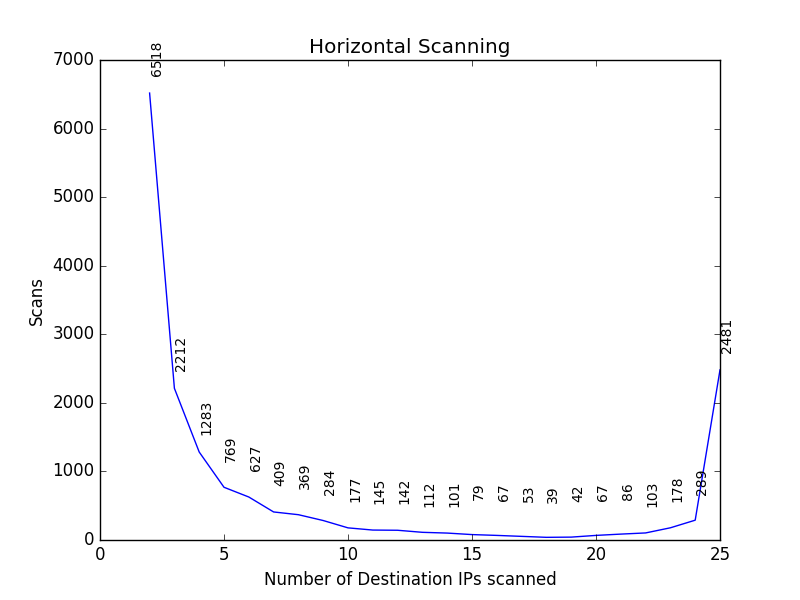
\includegraphics[width=1\linewidth]{images/horizontal_scans_jan_classc}
  \caption{TCP horizontal scanning grouped by same /24 network(without honeypot)}
  \label{fig:test1}
\end{minipage}%
\begin{minipage}{.535\textwidth}
  \centering
  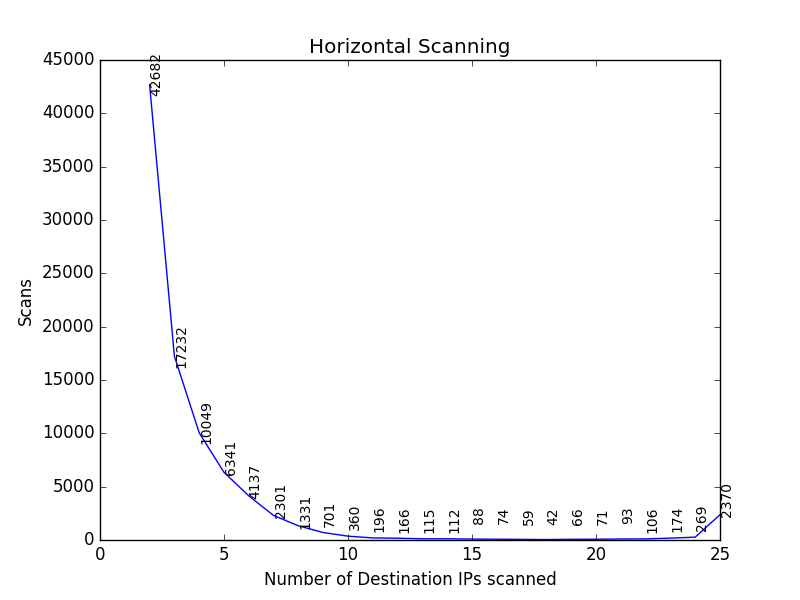
\includegraphics[width=1\linewidth]{images/horizontal_scans_jan_isp}
  \caption{TCP horizontal scanning grouped by same ISP (without honeypot)}
  \label{fig:test2}
\end{minipage}
\end{figure}
\\\\
Figure 7.2 shows the similar graph as explained in the above paragraph, but grouped by same ISP for the initial configuration (without honeypot).
The reason for grouping the horizontal scans by these methods were explained in the section 4.2.
It is clear from Figure 7.2 that, it shows similar behavior as first graph.
Nevertheless, the number of horizontal scans are increased in general for each corresponding horizontal scan size as compared to first graph.
This is due to the fact that, in the second approach, we  consider a very broader perspective by assuming that possibly all attacks from same source come from the same Internet Service Provider (ISP).
So this approach is used to minimize error, but the chances of including the false positives are high.
\begin{figure}[ht]
\captionsetup{justification   = raggedright,
              singlelinecheck = false}
\centering
\begin{minipage}{.535\textwidth}
  \centering
  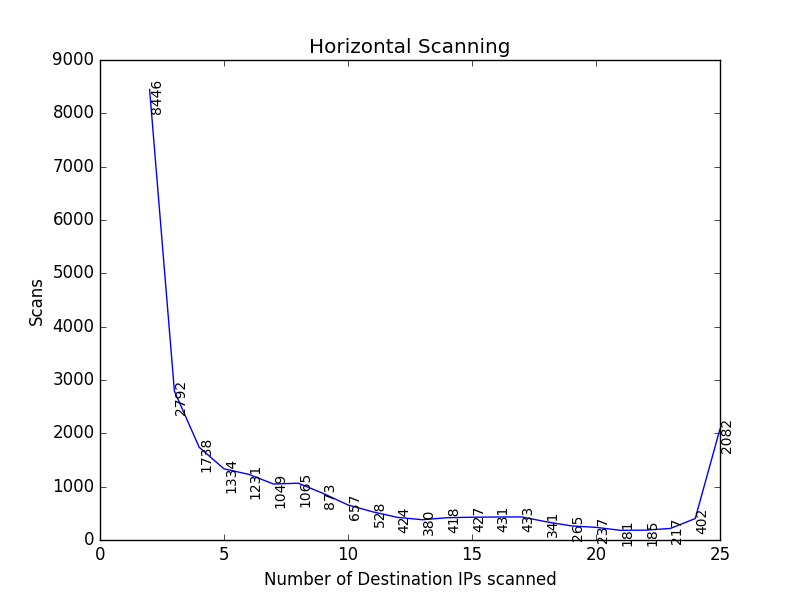
\includegraphics[width=1\linewidth]{images/horizontal_scans_march_classc}
  \caption{TCP horizontal scanning grouped by same /24 network (with honeypot)}
  \label{fig:march_classc}
\end{minipage}%
\begin{minipage}{.535\textwidth}
  \centering
  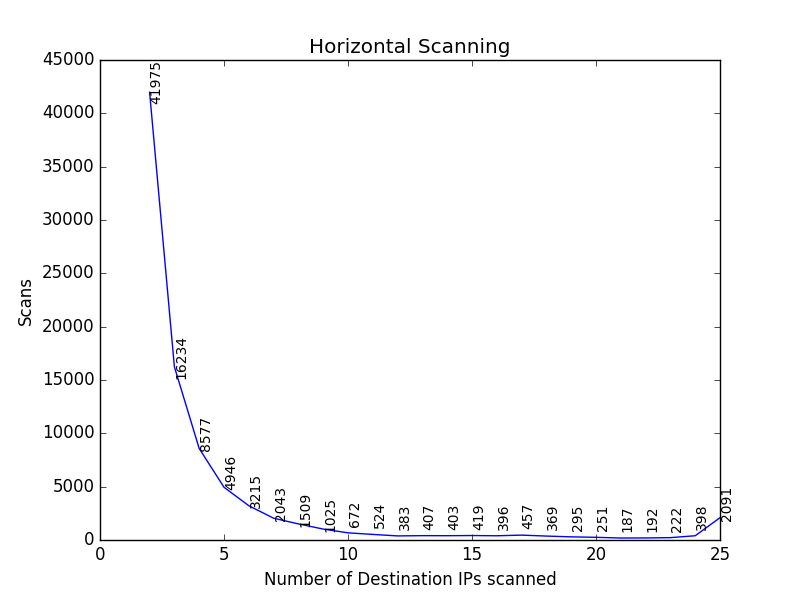
\includegraphics[width=1\linewidth]{images/horizontal_scans_march_isp}
  \caption{TCP horizontal scanning grouped by same ISP (with honeypot)}
  \label{fig:march_isp}
\end{minipage}
\end{figure}
\\\\
Figure 7.3 and Figure 7.4 show the correlation of horizontal scan sizes and number of horizontal scans for the second configuration (with honeypot) grouped by same /24 network and same ISP respectively.
These graphs show similar behavior compared to horizontal scanning graphs plotted by analysing the dataset obtained using network telescope without honeypot.
However it is not very easy to compare the behavior of horizontal scanning with regards to the total number of horizontal scans, as it is larger at second dataset when the scans are grouped by same /24 network but, number of scans is more at first dataset when it is grouped by same ISP.
Examining overall pattern of above mentioned graphs, number of horizontal scans keep reducing when number of distinct destination IP's scanned by scan source increases.
\\\\
Figure 7.5 illustrates the correlation between vertical scans sizes (number of distinct destination ports scanned) and number of vertical scans in TCP port scans for the initial configuration (without honeypot) grouped by same /24 network.
Using this graph and the Table 7.3, we can understand that around 94\% of total vertical scans have been obtained at vertical scan size 2.
It falls dramatically to about 3\% at vertical scan size 3 and it keep decreasing gradually when vertical scan size increases.
Finally number of vertical scans drop to single digit  at vertical scan sizes 79 and 82. 
The graph clearly shows that number of vertical scans get decreasing when the vertical scan size increases.\\\\
Figure 7.6 shows the similar graph as explained in the above paragraph, but grouped by same ISP for the initial configuration (without honeypot).
This graph shows similar behavior as first graph.
However total number of vertical scans have been increased very much compared to first graph and 88\% of the total vertical scans have been shown at vertical scan size 2.
It is interesting to notice that 99\% of the total scans have been obtained before vertical scan size reached 10 in both graphs.
Moreover number of vertical scans is same in both graphs after vertical scan size becomes 10.
These scans were originated from only 4 class C networks such as 185.40.4.0/24, 212.71.238.0/24, 183.3.227.0/24 and 62.210.246.0/24.
In the second graph false positives might have included in the initial values of vertical scan size since difference between number of vertical scans in the first and second graphs keep reducing when vertical scan size increases.
\\\\
\begin{figure}[p]
\centering
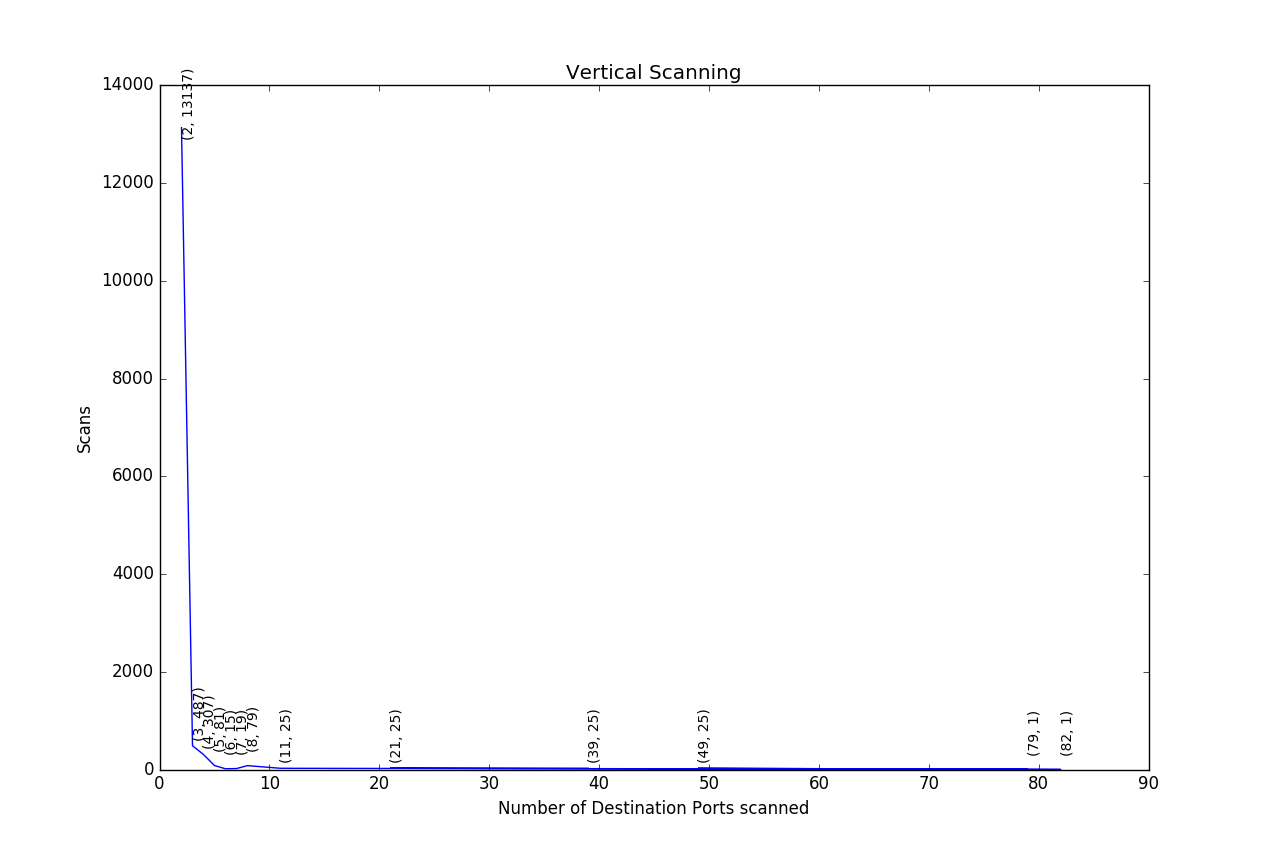
\includegraphics[width=15cm,height=9cm]{images/vertical_scans_jan_classc}
\caption{ TCP vertical scanning grouped by same /24 network (without honeypot)}
\centering
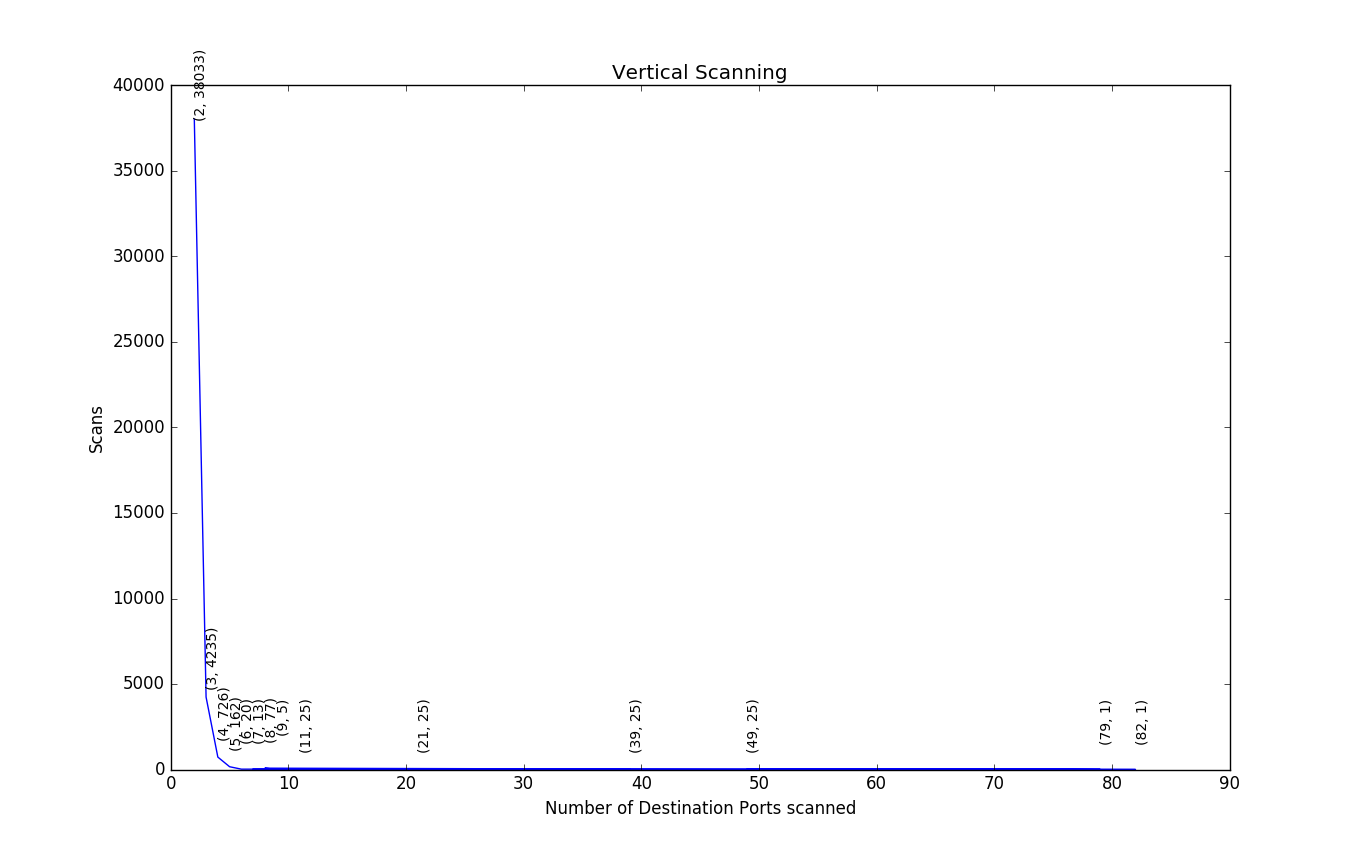
\includegraphics[width=15cm,height=9cm]{images/vertical_scans_jan_isp}
\caption{ TCP vertical scanning grouped by same ISP (without honeypot)}
\end{figure}
\begin{figure}[p]
\centering
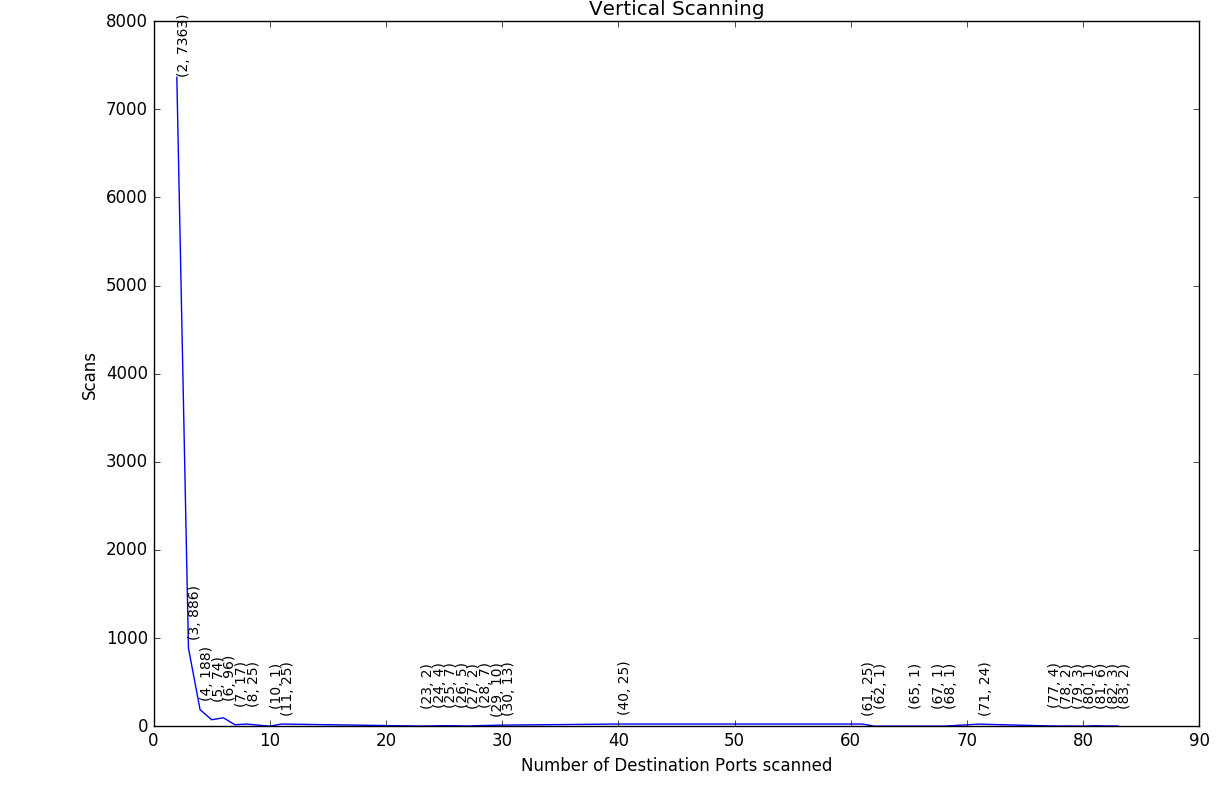
\includegraphics[width=15cm,height=9cm]{images/vertical_scans_march_classc}
\caption{ TCP vertical scanning grouped by same /24 network (with honeypot)}
\centering
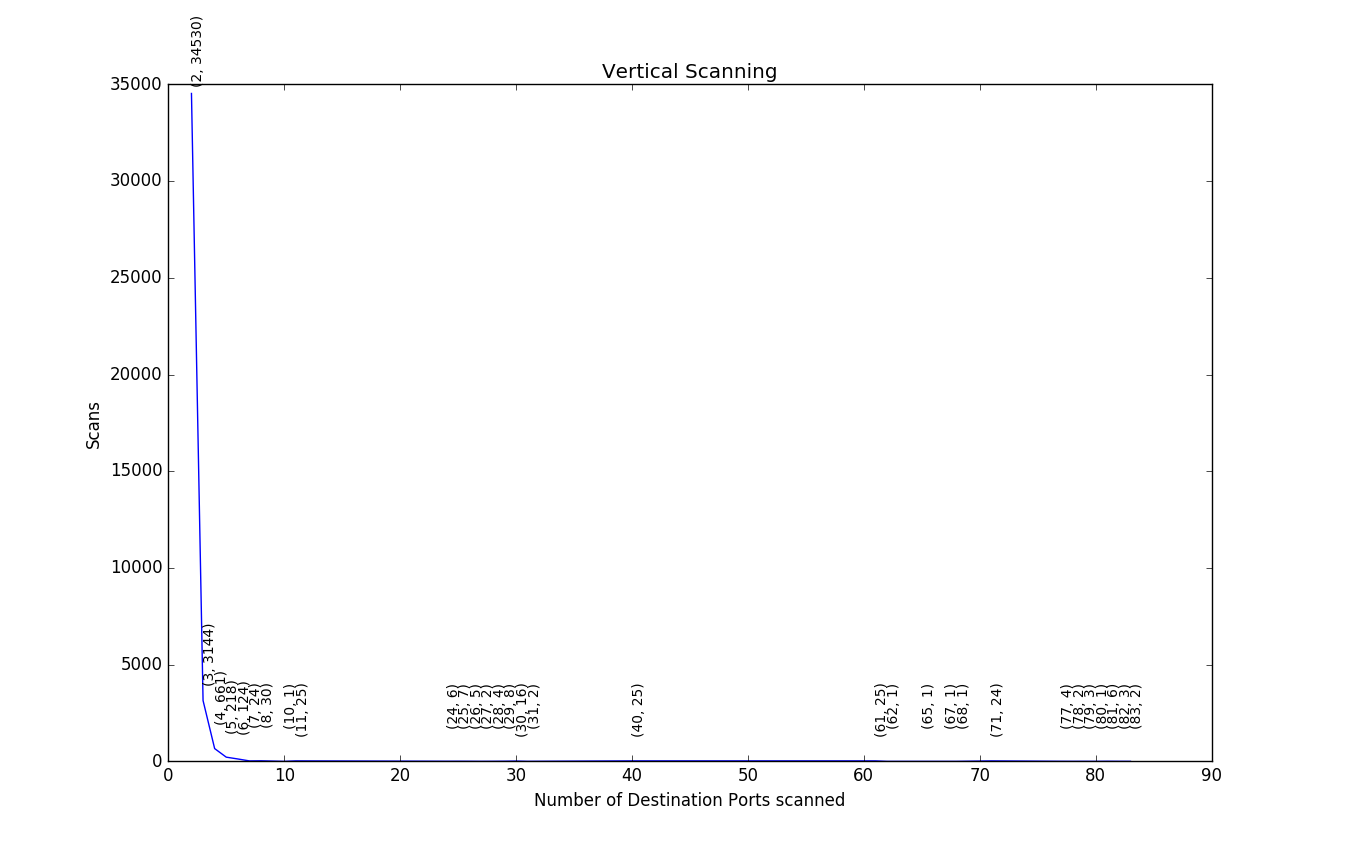
\includegraphics[width=16.5cm,height=9cm]{images/vertical_scans_march_isp}
\caption{ TCP vertical scanning grouped by same ISP (with honeypot)}
\end{figure}
\newpage
\noindent
Figure 7.7 and Figure 7.8 show the correlation of vertical scans sizes and number of vertical scans in TCP port scans for the second configuration (with honeypot) grouped by same /24 network and same ISP respectively. 
These graphs show similar behavior compared to vertical scanning graphs plotted by analysing the dataset obtained using network telescope without honeypot. 
In the Figure 7.7, around 83\% of total vertical scans have been obtained at vertical scan size 2 and it falls to around 6\% at vertical scan size 3.
As similar to graph explained in previous paragraph, number of vertical scans keep decreasing gradually when vertical scan size increases.
In the Figure 7.8, total number of vertical scans have been increased very much compared to first graph.
Similar to vertical scanning graphs obtained using first dataset, number of vertical scans is same in both graphs after vertical scan size becomes 10.
Vertical scans which are targeted on more than 10 destination ports are coming from mainly four countries: China, United States, France and Switzerland.
Moreover these scans are originated from only 6 class C networks such as 113.240.250.0/24 , 69.64.33.0/24, 222.186.34.0/24, 163.172.99.0/24, 193.138.215.0/24 and 173.254.236.0/24 at multiple times during this time span.\\\\ 
From the above mentioned four graphs,  we can see that there are small number
of large scans, with the size distribution being dominated by small scans.
However, number of large scans in the graphs from the second configuration (with honeypot) have been increased in general compared to graphs from the first configuration.
In addition to that, number of different vertical scan sizes have been also increased in the graphs obtained at second configuration compared to graphs from the first configuration.
\subsubsection{Horizontal and Vertical Scanning in UDP Port Scans}
Table 7.5 illustrates number of horizontal and vertical scans in UDP scans for two datasets and its counts. 
Number of horizontal and vertical scanning in UDP port scans are less compare to the corresponding values in TCP port scans.
Moreover, similar to Table 7.3, horizontal and vertical scanning counts are high when it is grouped by same ISP compared to when it is grouped by same /24 network in both first and second configuration.
\begin{table}[t!]
    \centering
    \resizebox{\columnwidth}{!}{%
    \begin{tabular}{c|c|c|c|}
    \hline
    \multicolumn{1}{ |c| }{Network Telescope Configuration}& Grouping & Number of Horizontal scans & Number of Vertical scans  \\ \cline{1-4}
    \multicolumn{1}{ |c  }{\multirow{2}{*}{Without Honeypot} } &
    \multicolumn{1}{ |c| }{same /24 network} & 7801 & 1715  \\ \cline{2-4}
    \multicolumn{1}{ |c  }{}                        &
    \multicolumn{1}{ |c| }{same ISP} & 11130 & 2612   \\ \cline{1-4}   
    \multicolumn{1}{ |c  }{\multirow{2}{*}{With Honeypot} } &
    \multicolumn{1}{ |c| }{same /24 network} & 9080 & 1158 \\ \cline{2-4}
    \multicolumn{1}{ |c  }{}  &
    \multicolumn{1}{ |c| }{same ISP} & 10794 & 2318   \\ \cline{1-4}   
    \end{tabular}
    }
    \caption{Number of Horizontal and Vertical scans in UDP Port Scans for Two Datasets and its Counts}
\end{table}
\begin{figure}
\captionsetup{justification   = raggedright,
              singlelinecheck = false}
\centering
\begin{minipage}{.535\textwidth}
  \centering
  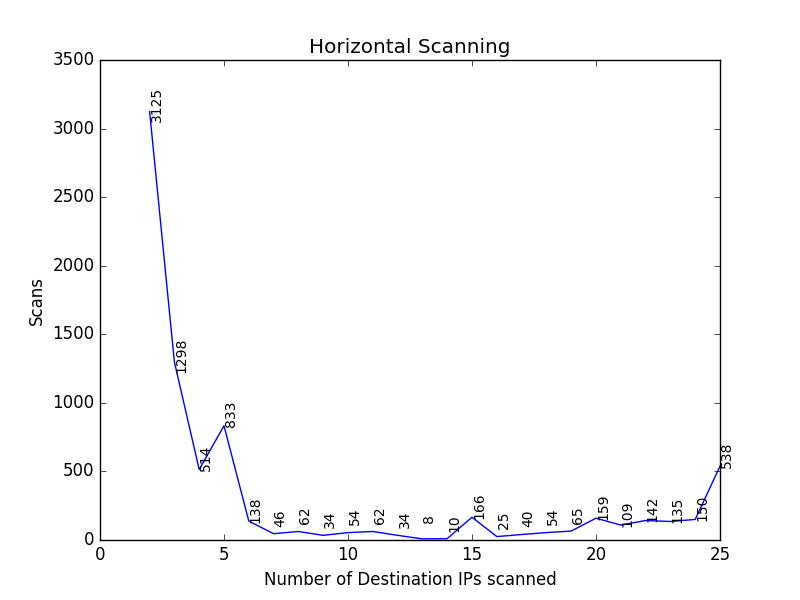
\includegraphics[width=1\linewidth]{images/horizontalscan_udp_classc}
  \caption{UDP horizontal scanning grouped by same /24 network(without honeypot)}
  \label{fig:horizontalscanningudpsameclassc}
\end{minipage}%
\begin{minipage}{.535\textwidth}
  \centering
  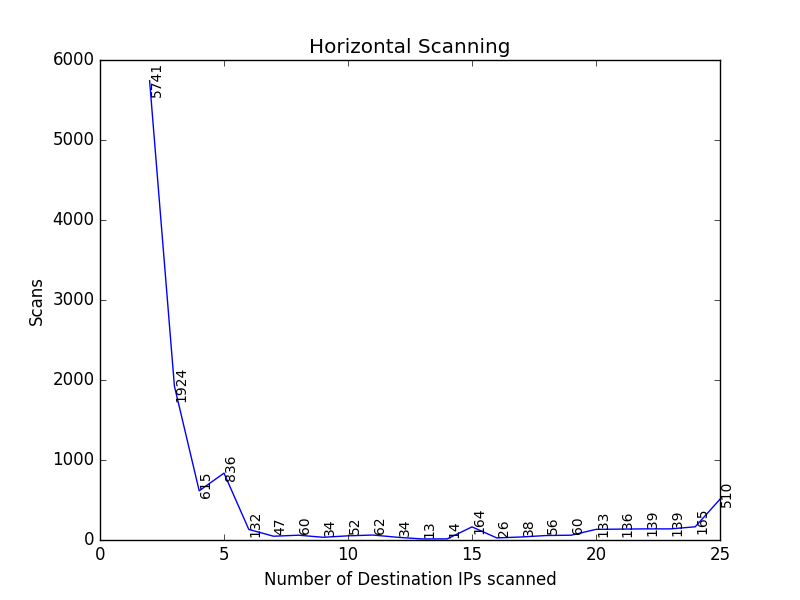
\includegraphics[width=1\linewidth]{images/horizontalscan_udp_isp_first}
  \caption{UDP horizontal scanning grouped by same ISP (without honeypot)}
  \label{fig:horizontalscanningudpsameisp}
\end{minipage}
\end{figure}
\\\\
Figure 7.9 and Figure 7.10 show the correlation of horizontal scan sizes and number of horizontal scans in UDP port scans for first configuration (without honeypot) grouped by same /24 network and same ISP respectively.
Overall, similar to behavior of  horizontal scanning graphs for TCP port scans shown in Figure 7.1 and 7.2, the number of horizontal scans are decreased in respect to increase of number of destination IPs scanned.
However, number of horizontal scans are less in general for each corresponding horizontal scan size as compared to graphs in Figure 7.1 and 7.2.
\begin{figure}[h!]
\captionsetup{justification   = raggedright,
              singlelinecheck = false}
\centering
\begin{minipage}{.535\textwidth}
  \centering
  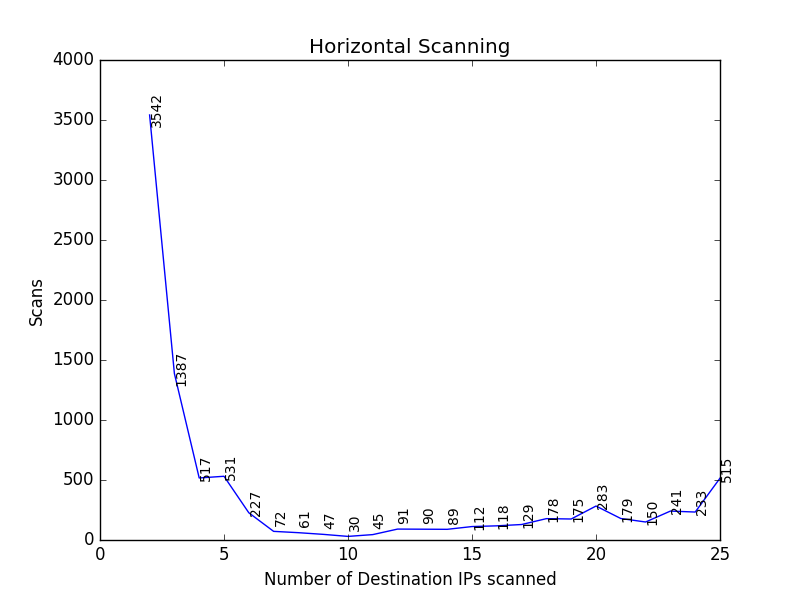
\includegraphics[width=1\linewidth]{images/horizontalscan_udp_classc_honeypot}
  \caption{UDP horizontal scanning grouped by same /24 network(with honeypot)}
  \label{fig:horizontalscanningudpsameclasscwithhoneypot}
\end{minipage}%
\begin{minipage}{.535\textwidth}
  \centering
  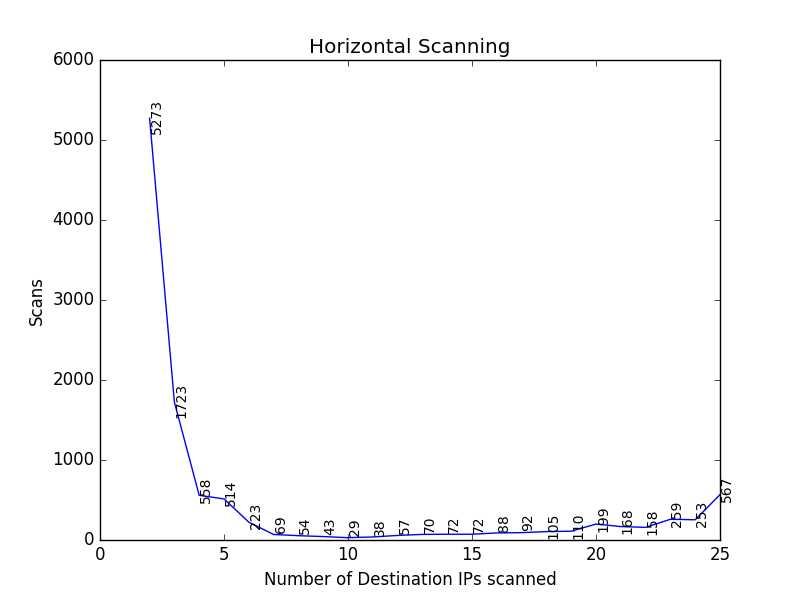
\includegraphics[width=1\linewidth]{images/horizontalscan_udp_isp_honeypot}
  \caption{UDP horizontal scanning grouped by same ISP (with honeypot)}
  \label{fig:horizontalscanningudpsameispwithhoneypot}
\end{minipage}
\end{figure}
\\\\
Figure 7.11 and Figure 7.12  show the correlation of horizontal scan sizes and number of horizontal scans in UDP port scans for the second configuration (with honeypot) grouped by same /24 network and same ISP respectively.
These graphs also show similar behavior compared to  horizontal scanning graphs for TCP port scans shown in Figure 7.3 and 7.4.
Nevertheless, number of horizontal scans are less in general for each corresponding horizontal scan size as compared to graphs in Figure 7.3 and 7.4.
Nevertheless, number of horizontal scans are less in general for each corresponding horizontal scan size as compared to graphs in Figure 7.3 and 7.4.
\begin{figure}[p]
\centering
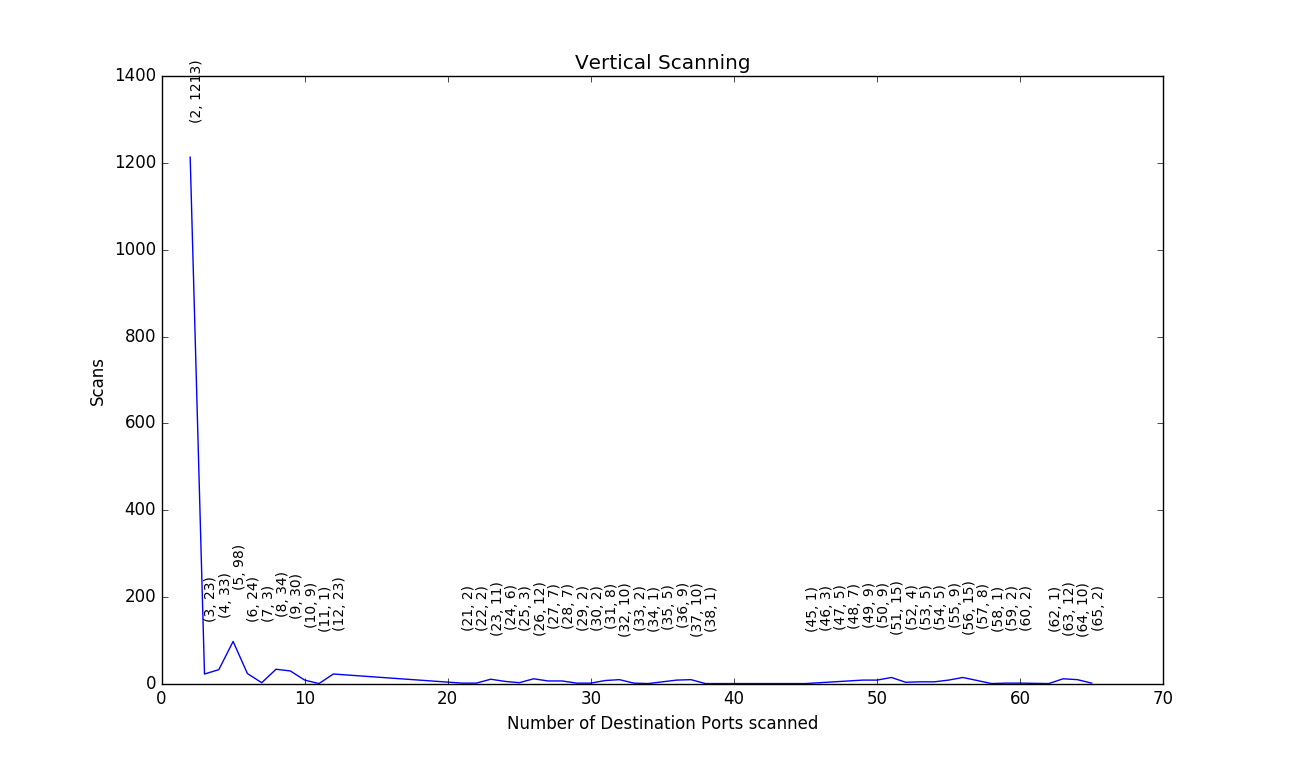
\includegraphics[width=15cm,height=9cm]{images/verticalscan_udp_classc}
\caption{ UDP vertical scanning grouped by same /24 network (without honeypot)}
\centering
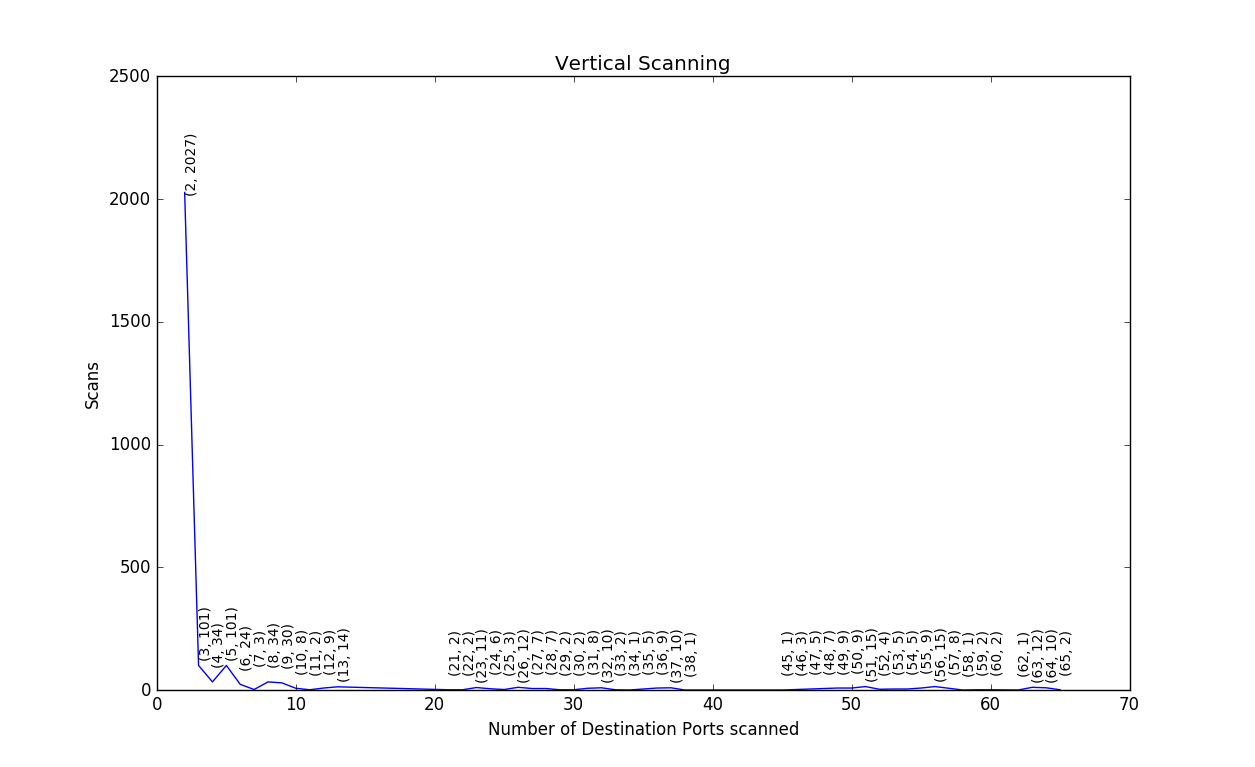
\includegraphics[width=15cm,height=9cm]{images/verticalscan_udp_isp_first}
\caption{ UDP vertical scanning grouped by same ISP (without honeypot)}
\end{figure}
\\\\
Figure 7.13 and Figure 7.14 show the correlation of vertical scans sizes and number of vertical scans in UDP scans for the first configuration (without honeypot) grouped by same /24 network and same ISP respectively.
From Figure 7.13 and Table 7.5, we can understand that around 71\% of total vertical scans have been obtained at vertical scan size 2.
In Figure 7.14, around 78\% of total vertical scans have been obtained at vertical scan size 2.
Similar to graphs plotted in Figure 7.5 and 7.6, these graphs also show that number of vertical scans get decreasing in general when the vertical scan size increases.
Moreover, it is interesting to notice that number of vertical scans is same in both graphs after vertical scan size 20. 
It is because all these port scans were generated from only one source IP address which is 104.193.11.107.
From the explanation given for Figure 7.5 and 7.6,  it is understood that this IP address (104.193.11.107) did not participate in TCP vertical scans which target on more than 20 destination ports during the same time period.
\begin{figure}[p]
\centering
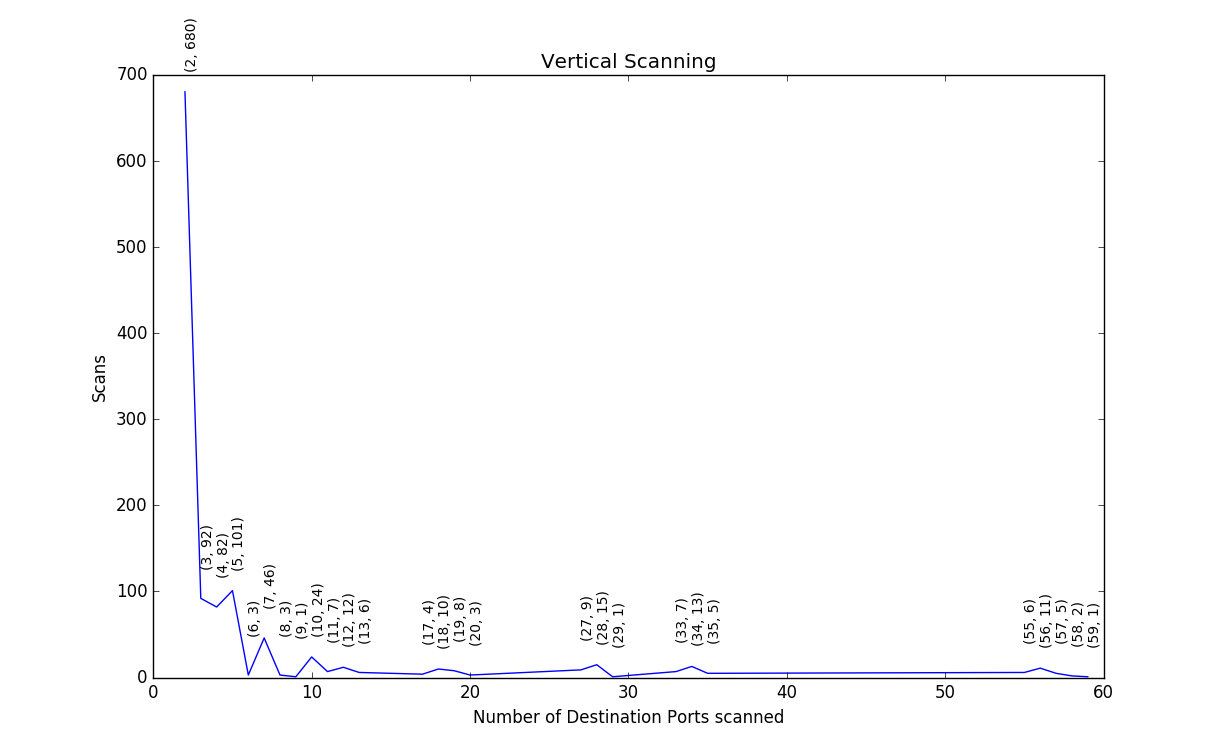
\includegraphics[width=15cm,height=9cm]{images/verticalscan_udp_classc_honeypot}
\caption{ UDP vertical scanning grouped by same /24 network (with honeypot)}
\centering
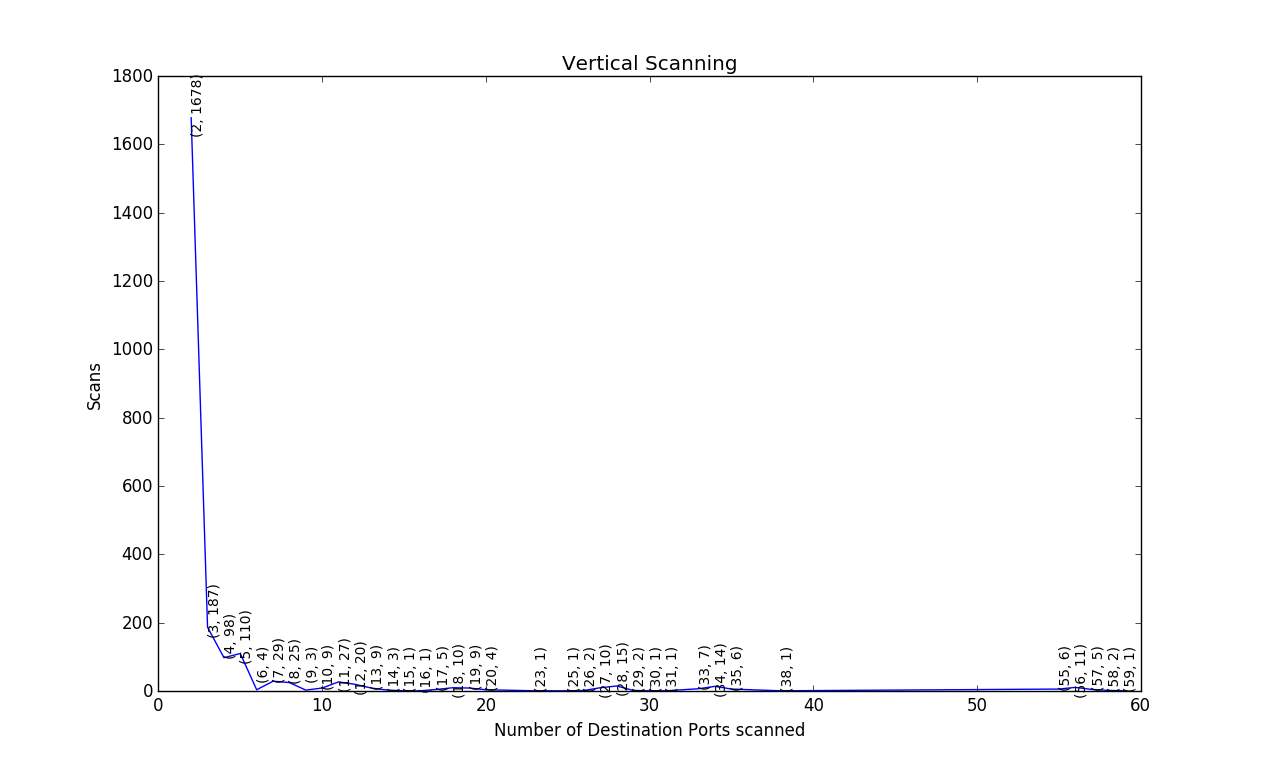
\includegraphics[width=16.5cm,height=9cm]{images/verticalscan_udp_isp_honeypot}
\caption{ UDP vertical scanning grouped by same same ISP (with honeypot)}
\end{figure}
\\\\
Figure 7.15 and Figure 7.16 show the correlation of vertical scans sizes and number of vertical scans in UDP port scans for the second configuration (with honeypot) grouped by same /24 network and same ISP respectively.
These graphs show similar behavior compared to  vertical scanning graphs for TCP port scans shown in Figure 7.7 and 7.8.
Similar to analysis results obtained in previous paragraph, more than half amount of total vertical scans have been received at vertical scan size 2 for both graphs plotted in Figure 7.15 and 7.16.
However, number of vertical scans which is targeted on more than 20 destination ports are less during second configuration compared to same value in first configuration.
While comparing the source IPs targeted on more than 20 destination ports for TCP and UDP vertical scans, we can see that
source IPs who perform large scans at TCP and UDP ports are different.
From the graphs plotted for the analysis of vertical scans in UDP port scans, we can understand that there are small number of large scans, with the size distribution being dominated by small scans as similar to the results of TCP port scans. 
\subsection{Target Ports}
The popularity of target ports for TCP and UDP packets was another metric we evaluated during the analysis of dataset obtained from first and second configuration.
We analysed captured packets from these two configurations and compared the behavior of port scan activity based on targeted ports.\\\\
\newpage 
\noindent
In the first dataset, out of total 65536 port numbers, only  913 TCP ports were scanned at least once during this time span.
As some of the ports were scanned only once during this time span, around 93\% of the ports were scanned many more times during this period.
Table 7.5 lists the top 20 most actively scanned TCP ports, the corresponding services and some related statistics from dataset obtained at first configuration.
We can see that more than half of the total TCP scans were targeted on port 23.
Port 22 was scanned more than 6\% of the total port scans.
 \begin{table}[t!]
    \centering
    \scalebox{0.7}{
    \begin{tabular}{ |c|c|c|c| }
     \hline
     \textbf{Port Number} & \textbf{Number Of Hits} & \textbf{Percentage of Total} & \textbf{Port Services} \\
     \hline
     23 & 371626 & 51.7 & Telnet\\ 
     \hline
     22 & 52303 & 6.5 & SSH \\ 
     \hline
    7547 & 47551 & 5.9 & \makecell{TR-069 -Application layer protocol for  \\ remote management of end-user devices.}\\
    \hline
    2323 & 32002 &  4.5 & \makecell{3d-nfsd - Special file system for\\ controlling Linux NFS server} \\ 
    \hline
    6789 & 34422 & 4.3  & IBM db2 web control center\\
    \hline
    23231 & 32053 & 4  & Unassigned\\ 
    \hline
    5358 & 27571 &  3.4 &wsdapi-s - Web Services for Devices Secured port\\ 
    \hline
    1433 & 18936 &  2.4 &SMC-HTTPS\\ 
    \hline
    443 & 15792 &  2.1 &HTTP protocol over TLS/SSL\\ 
    \hline
    37777 &  10216 &  1.2 &Digital Video Recorder hardware\\ 
    \hline
    3389 & 9247&  1.1 & \makecell{Microsoft Terminal Server (RDP) officially \\ registered as Windows Based Terminal (WBT)}\\
    \hline
    80 & 6976 & 0.87 &HTTP\\
    \hline
    8080 &  5826&  0.73 &HTTP Alternate\\ 
    \hline
    3306 & 5229 & 0.65 &Microsoft Directory Services\\ 
    \hline
    2222 &  4720&  0.59 &Rockwell CSP2\\ 
    \hline
    1099 &  2196&  0.27 &RMI Registry\\ 
    \hline
    445 &  1921 & 0.24 &Microsoft Directory Services\\ 
    \hline
    5900 &  1856&  0.23 &Virtual Network Computing (VNC)-  remote
control program\\ 
    \hline
    21 & 1564 & 0.19 &FTP - File Transfer Protocol\\
    \hline
    81 & 1480 & 0.18 & HTTP Alternate\\ 
    \hline
    \end{tabular}
    }
    \caption{Top 20: Most Actively Scanned TCP Ports and their Functions without Honeypot}
\end{table}
\begin{table}[t!]
    \centering
    \scalebox{0.7}{
    \begin{tabular}{ |c|c|c|c| } 
     \hline
    \textbf{Port Number} & \textbf{Number Of Hits} & \textbf{Percentage of Total} & \textbf{Port Services} \\
     \hline
     23 & 315374 & 39.6 & Telnet\\ 
     \hline
     22 & 120980 & 15.2 & SSH \\ 
     \hline
    5358 & 70943 & 8.9 &wsdapi-s - Web Services for Devices Secured port\\
    \hline
    7547 & 49162 & 6.1 & \makecell{TR-069 -Application layer protocol for  \\ remote management of end-user devices.}\\
    \hline
    2323 & 23719 & 2.9& \makecell{3d-nfsd - Special file system for\\ controlling Linux NFS server} \\ 
    \hline
    443 & 17898 & 2.2 &HTTP protocol over TLS/SSL\\ 
    \hline
    80 & 14815 & 1.8 &HTTP\\
    \hline
     3389 & 11036 & 1.3 & \makecell{Microsoft Terminal Server (RDP) officially \\ registered as Windows Based Terminal (WBT)}\\
    \hline
    3306 & 8980 & 1.1 &Microsoft Directory Services\\ 
    \hline
    8080 &  8413 & 1.05 &HTTP Alternate\\ 
    \hline
    1433 & 7702 & 0.96 &SMC-HTTPS\\ 
    \hline
    2222 & 6181 & 0.77 & Rockwell CSP2\\
    \hline
    445 &   3078 & 0.38 &Microsoft Directory Services\\ 
    \hline
     21 & 3075 & 0.38 &FTP - File Transfer Protocol\\
    \hline
    81 & 2870 & 0.36 & HTTP Alternate\\ 
    \hline
    5900 &  2715 & 0.34 & Virtual Network Computing (VNC)- remote
    control program\\
    \hline
    25 & 2471 & 0.31 & Simple Mail Transfer Protocol (SMTP)\\
    \hline
    88 & 2185 & 0.27 & Kerberos Key Distribution Center (KDC) server\\
    \hline
    6789 & 1867 & 0.23  & IBM db2 web control center\\
    \hline
    3390 & 1798 & 0.22 & Trojans\\ 
    \hline
    \end{tabular}
    }
    \caption{Top 20: Most Actively Scanned TCP Ports and their Functions with Honeypot}
\end{table}
Most of the ports in the Table 7.5 run a service that can be exploited by attackers except port 23231 in which no popular service is assigned on.
When we studied more extensively about port 23231, we understand that the large number of port scans are due to Mirai vulnerability scanning activity.
Mirai vulnerability scanner scans the IP addresses to check if the target network hosts a device vulnerable to Mirai injection attacks \cite{hallman2017ioddos}.
Since there is no active service reside on port 23231, Figure 7.17 clearly shows that TCP connection includes only two packets and port 23231 is closed.
Moreover it shows that, there is no actual data being transferred between source and target system. 
\begin{figure}[ht]
\centering
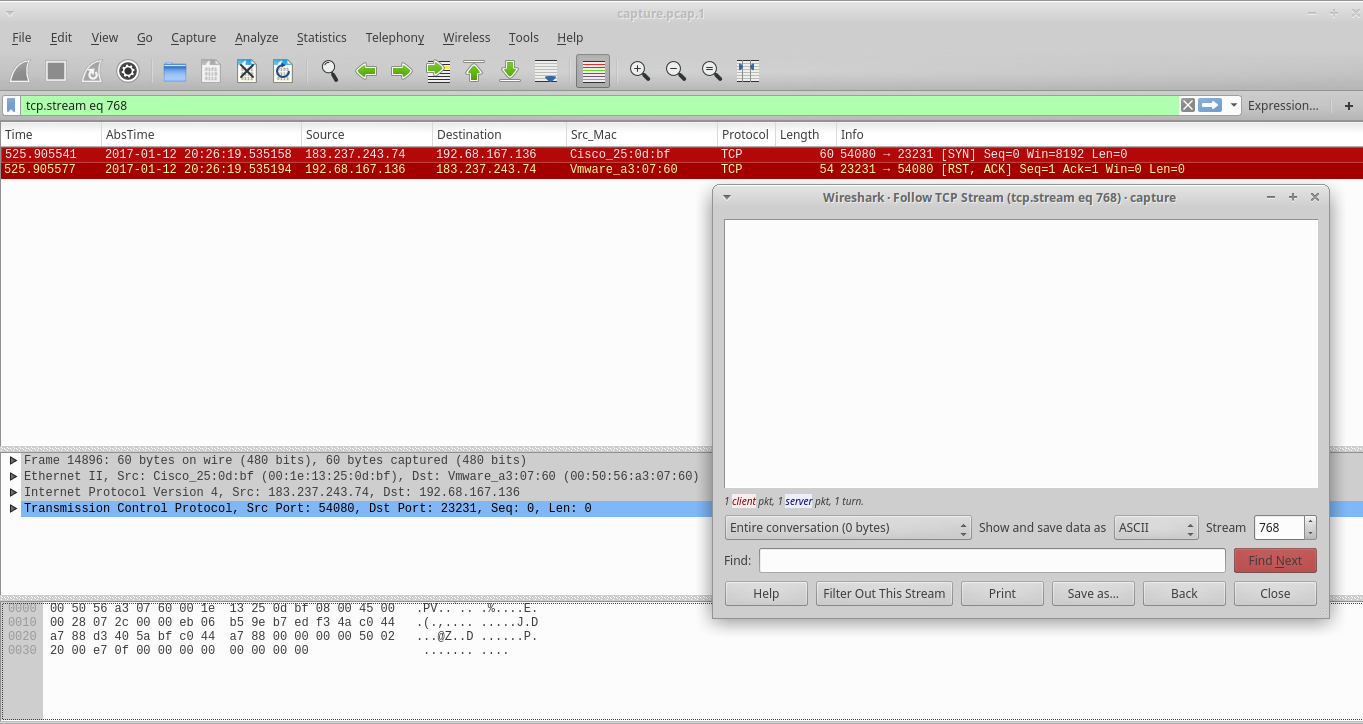
\includegraphics[width=16cm, height=10cm]{images/23231port.png}
\caption{TCP stream of port scan targeted on port 23231 shows that port is closed and there is no actual data being transferred between source and target system }
\end{figure}
\\\\
In the second dataset, out of total 65536 port numbers, 1295 TCP ports were scanned at least once during this time span.
Comparing the number of ports scanned at first and second configuration, there is 41\% of increase in second stage.
This is due to more number of large scans in the second configuration, thus more number of ports are scanned as we discussed while explaining the Figure 7.7.
Around 92\% of the ports were scanned many more times during this period and amount of scans targeted on ports only once are very less. 
Table 7.6 lists the top 20 most actively scanned TCP ports, the corresponding services and some related statistics from dataset obtained at second configuration.
We can see that nearly 40\% of the total TCP scans were targeted on port 23.
Port 22 was scanned more than 15\% of the total port scans.
All top 20 ports are well known for running some services which are vulnerable for attacks.\\\\
We also analysed most actively scanned UDP ports as part of thesis work.
In the first dataset, out of total  65536 UDP ports, 825 UDP ports were scanned at least once during this time period.
Around 81\% of the UDP ports were scanned multiple times during this time period.
While during second configuration, 2249 UDP ports were scanned at least once.
However only 19\% of these ports were scanned multiple times during this period.
Comparing the number of TCP and UDP ports scanned at first and second configuration, we can see that a large percentage of increase in scanned ports at dataset obtained using network telescope with honeypot.
\begin{table}[t!]
    \centering
    \scalebox{0.7}{
    \begin{tabular}{ |c|c|c|c| } 
     \hline
     \textbf{Port Number} & \textbf{Number Of Hits} & \textbf{Percentage of Total} & \textbf{Port Services} \\
     \hline
     1900 & 23123 & 24.9& UPnP Simple Service Discovery Protocol (SSDP)\\
     \hline
     5060 & 22061 & 23.7 & Session Initiation Protocol (SIP)\\
     \hline
     161 & 5283 & 5.6 & SNMP\\
     \hline
     53413 & 4043 & 4.3 & Netis Router Backdoor\\
     \hline
     123 & 3528 & 3.8 & Network Time Protocol(NTP)\\
     \hline
    53 & 2739 & 2.9& DNS\\
    \hline
    2425 & 2427 & 2.6 & Fujitsu App Manager\\
    \hline
    137 & 1699 & 1.8 & Netbios\\
    \hline
    1434 & 1334 & 1.4 & Microsoft SQL Server\\
    \hline
    19 & 1000 & 1.07 & Character Generator Protocol(CHARGEN)\\
    \hline
    \end{tabular}
    }
    \caption{Top 10: Most Actively Scanned UDP Ports and their Functions without Honeypot}
\end{table}
\begin{table}[t!]
    \centering
    \scalebox{0.7}{
    \begin{tabular}{ |c|c|c|c| } 
     \hline
     \textbf{Port Number} & \textbf{Number Of Hits} & \textbf{Percentage of Total} & \textbf{Port Services} \\
     \hline
     5060 & 47292 & 42.8 & Session Initiation Protocol (SIP)\\
     \hline
     1900 &16463 & 14.9 & UPnP Simple Service Discovery Protocol (SSDP)\\
     \hline
     161 & 6728 & 6.1 & SNMP\\
     \hline
     53413 & 5451 & 4.9 & Netis Router Backdoor\\
    \hline
    123 & 3752 & 3.4 &Network Time Protocol(NTP)\\ 
     \hline
     53 & 3402 & 3.08 & DNS\\
    \hline
    137 & 1870 & 1.6 & Netbios\\
    \hline
    1434 & 1457 & 1.3 & Microsoft SQL Server\\
    \hline
    2425 & 1348 & 1.2 & Fujitsu App Manager\\
    \hline
    19 &1279 &1.1& Character Generator Protocol(CHARGEN)\\ 
    \hline
    \end{tabular}
    }
    \caption{Top 10: Most Actively Scanned UDP Ports and their Functions with Honeypot}
\end{table}
\\\\
Table 7.7 and Table 7.8 illustrate most actively scanned UDP ports and its function from dataset obtained at first and second configuration respectively.
All the top 10 ports are same in both Tables which show that these ports were most actively scanned ports irrespective of time period at which port scans were detected.
\subsection{Relationship between Traffic and Time of the Day}
Time distribution of port scan traffic for top 5 countries who participated in scanning activity was yet another metric we evaluated during the analysis of dataset obtained from first and second configuration.
We plotted a graph which shows the relationship between traffic rate and the time of the day for each country, to check if port scanning is a constant activity throughout the day or attackers are more interested in a particular time of the day to execute port scanning.\\\\
Figure 7.18 shows top 5 countries who participated in TCP port scanning activity and its traffic rate based on the local time of the source of attack from first configuration.
It is clear from the graph that, port scanning activity is a constant activity and graph does not show a correlation between traffic and time of the day.
In addition to that, Table 7.9 lists top 5 countries which involved in TCP port scanning activity at first configuration.  
\begin{figure}[p]
\centering
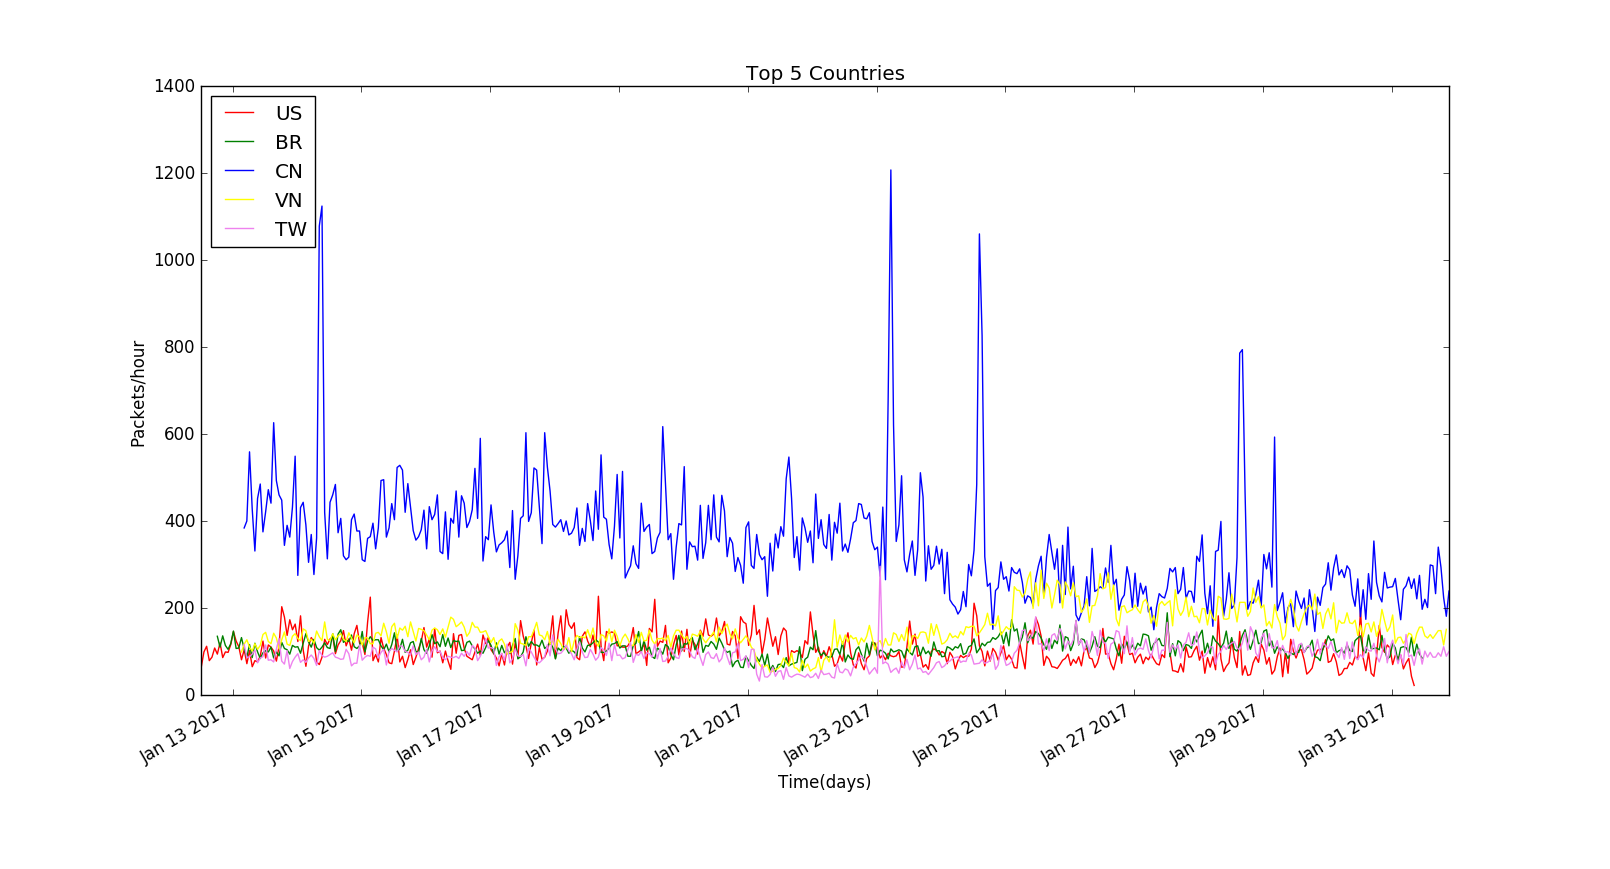
\includegraphics[width=16cm, height=9cm]{images/top5_countries_tcp_withouthoneypot1.png}
\caption{Top 5 countries participated in TCP port scanning activity and its traffic rate (first configuration)}
\centering
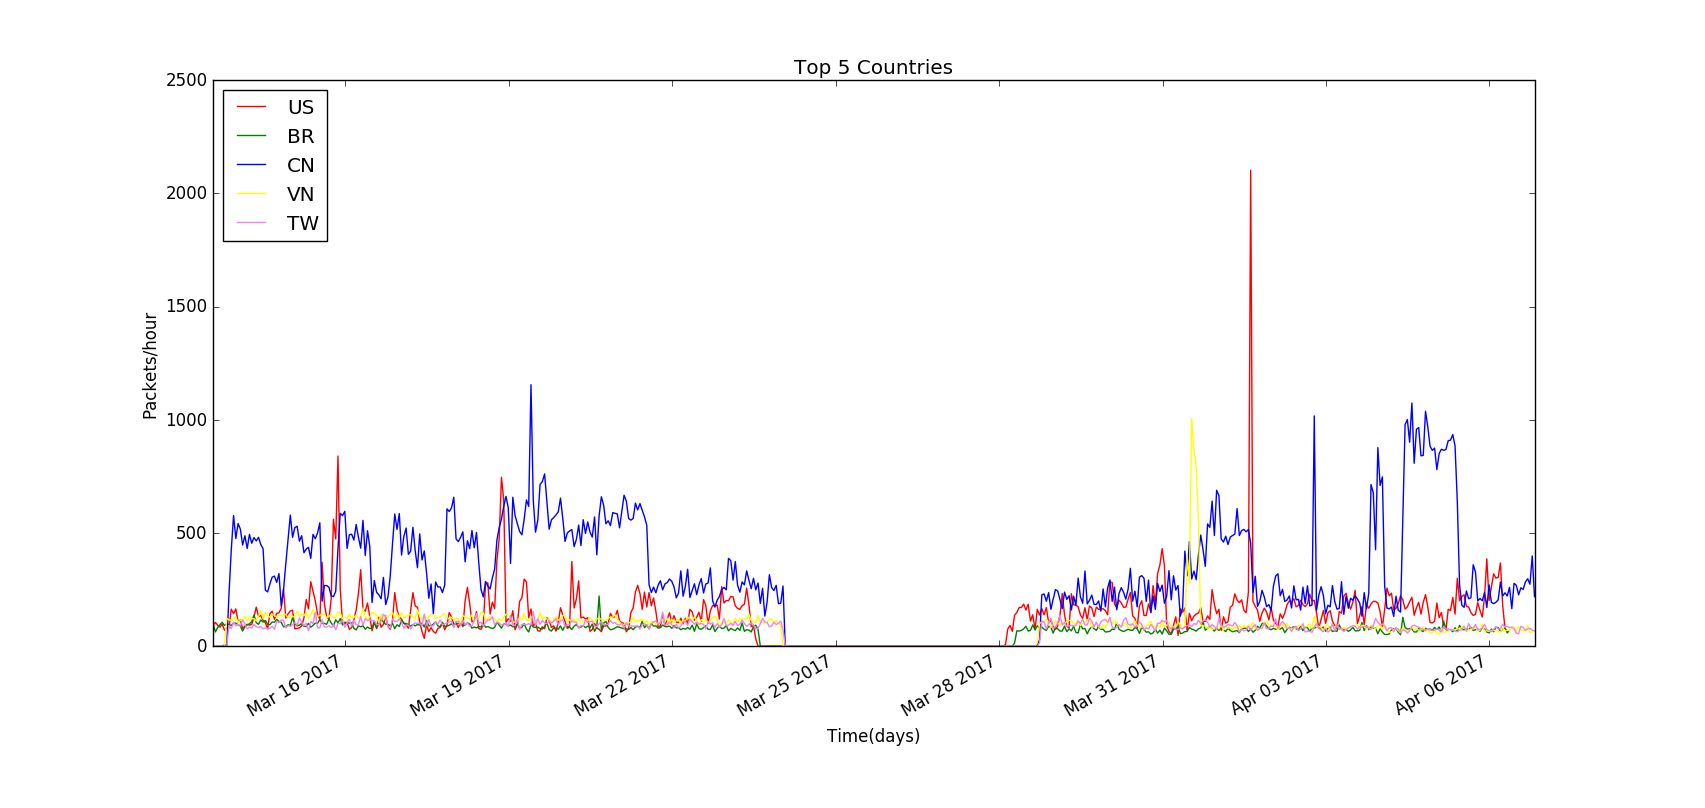
\includegraphics[width=16cm, height=9cm]{images/top5countries_tcp_march2.png}
\caption{Top 5 countries participated in TCP port scanning activity and its traffic rate (second configuration)}
\end{figure}
\begin{table}[t!]
    \centering
    \scalebox{0.7}{
    \begin{tabular}{ |c|c|c| } 
     \hline
     \textbf{Countries} & \textbf{Number of Scans} & \textbf{\% Total Scans} \\ 
     \hline
     China (CN) & 158366 & 19.9\\
     Vietnam (VN) & 68016 & 8.5\\
     United States (US) &  61874 & 7.7\\
     Brazil (BR)& 52167 & 6.5\\
     Taiwan (TW) & 42142 & 5.2\\
     \hline
    \end{tabular}
    }
    \caption{Top 5 countries participated in TCP port scanning activity at first configuration}
\end{table}
\begin{table}[t!]
    \centering
    \scalebox{0.7}{
    \begin{tabular}{ |c|c|c| } 
     \hline
     \textbf{Countries} & \textbf{Number of Scans} & \textbf{\% Total Scans} \\ 
     \hline
     China (CN) & 180169 & 22.3\\
     United States (US)& 93276 & 11.5\\
     Vietnam (VN) & 52076 & 6.4\\
     Brazil (BR) & 43279 & 5.3\\
     Taiwan (TW)& 40866 & 5.1\\
     \hline
    \end{tabular}
    }
    \caption{Top 5 countries participated in TCP port scanning activity at second configuration}
\end{table}
\\\\
Figure 7.19 shows top 5 countries who participated in TCP port scanning activity and its traffic rate based on the local time of the source of attack from second configuration.
Graph shows a similar behavior to the Figure 7.18 and port scanning is a constant activity in the second configuration also.
Table 7.10 illustrates top 5 countries which are involved in TCP port scanning activity at second configuration.
From Table 7.9 and 7.10, it is evident that top countries which involved in TCP port scans at both configurations are same.
\begin{figure}[p]
\centering
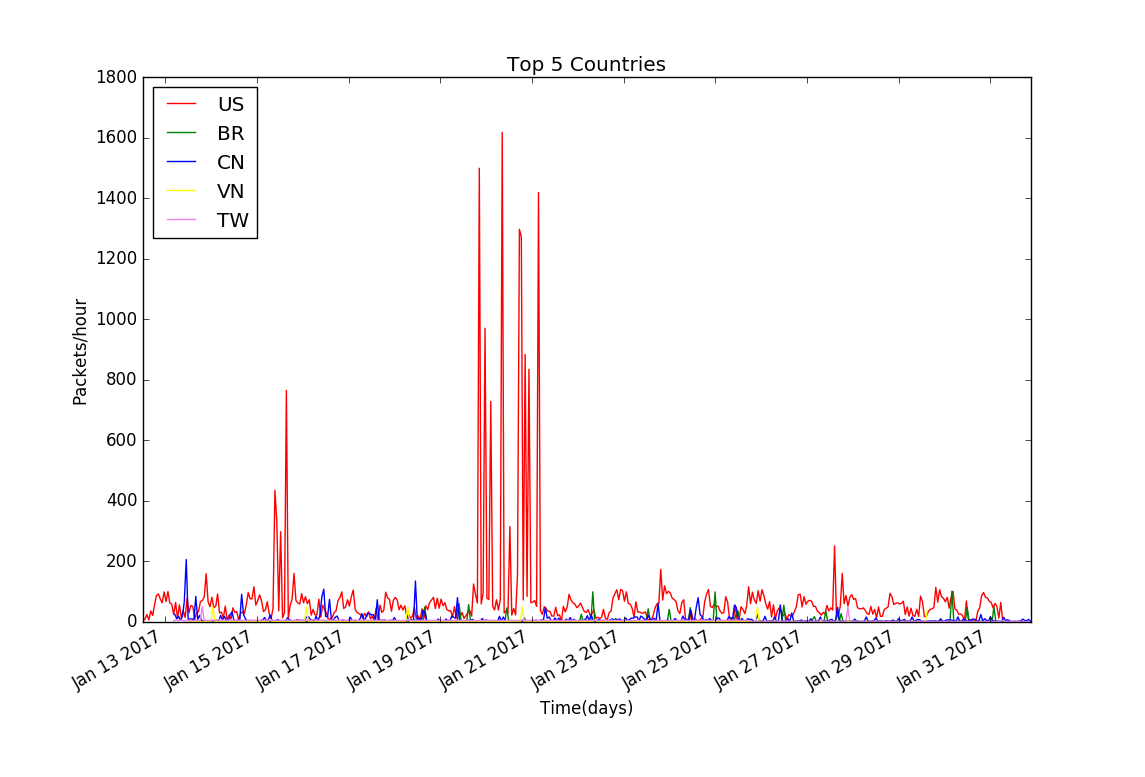
\includegraphics[width=15cm, height=9cm]{images/top5countries_udp_first.png}
\caption{Top 5 countries participated in UDP port scanning activity and its traffic rate (first configuration)}
\centering
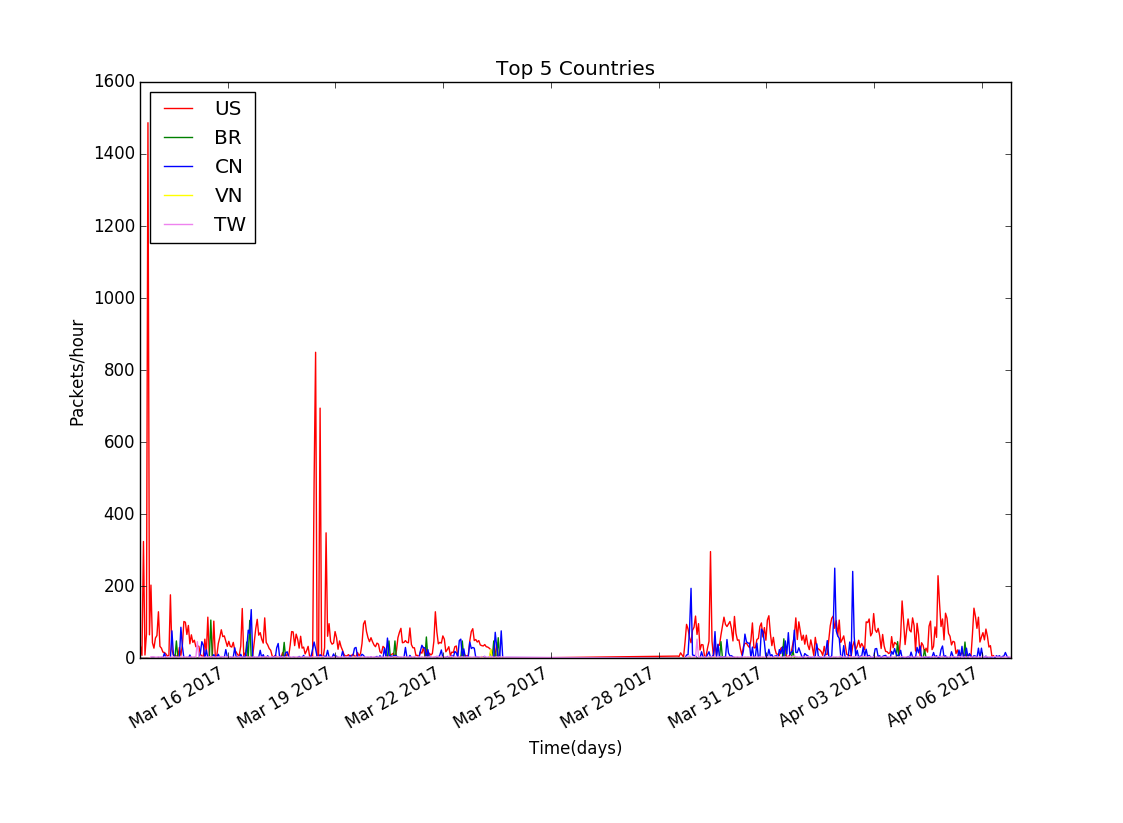
\includegraphics[width=15cm, height=9cm]{images/top5countries_udp_honeypot.png}
\caption{Top 5 countries participated in UDP port scanning activity and its traffic rate (second configuration)}
\end{figure}
\\\\
Figure 7.20 and Figure 7.21 show the graphs of top 5 countries who participated in UDP port scanning activity and its traffic rate based on the local time of the source of attack from first and second configuration respectively.
From these graphs, we can understand that UDP port scans are not very frequent as TCP port scanning activity.
However, UDP port scans do not show a correlation between traffic and time of the day as similar TCP port scanning activity.
Moreover, top 5 countries which are involved in UDP port scans at both first and second configuration are same and are China, United States, Vietnam, Brazil and Taiwan.
Another interesting fact is that, these are the top 5 countries which involved in TCP port scans as well.
\subsection{ Geographical Distribution of Port Scan Sources}
Another property we wanted to check is how port scan source IP addresses are geographically distributed around the world.
We implemented a method to do it by designing a heat map to show the geographical distribution of location of port scanning attacks.
\begin{figure}[p]
\centering
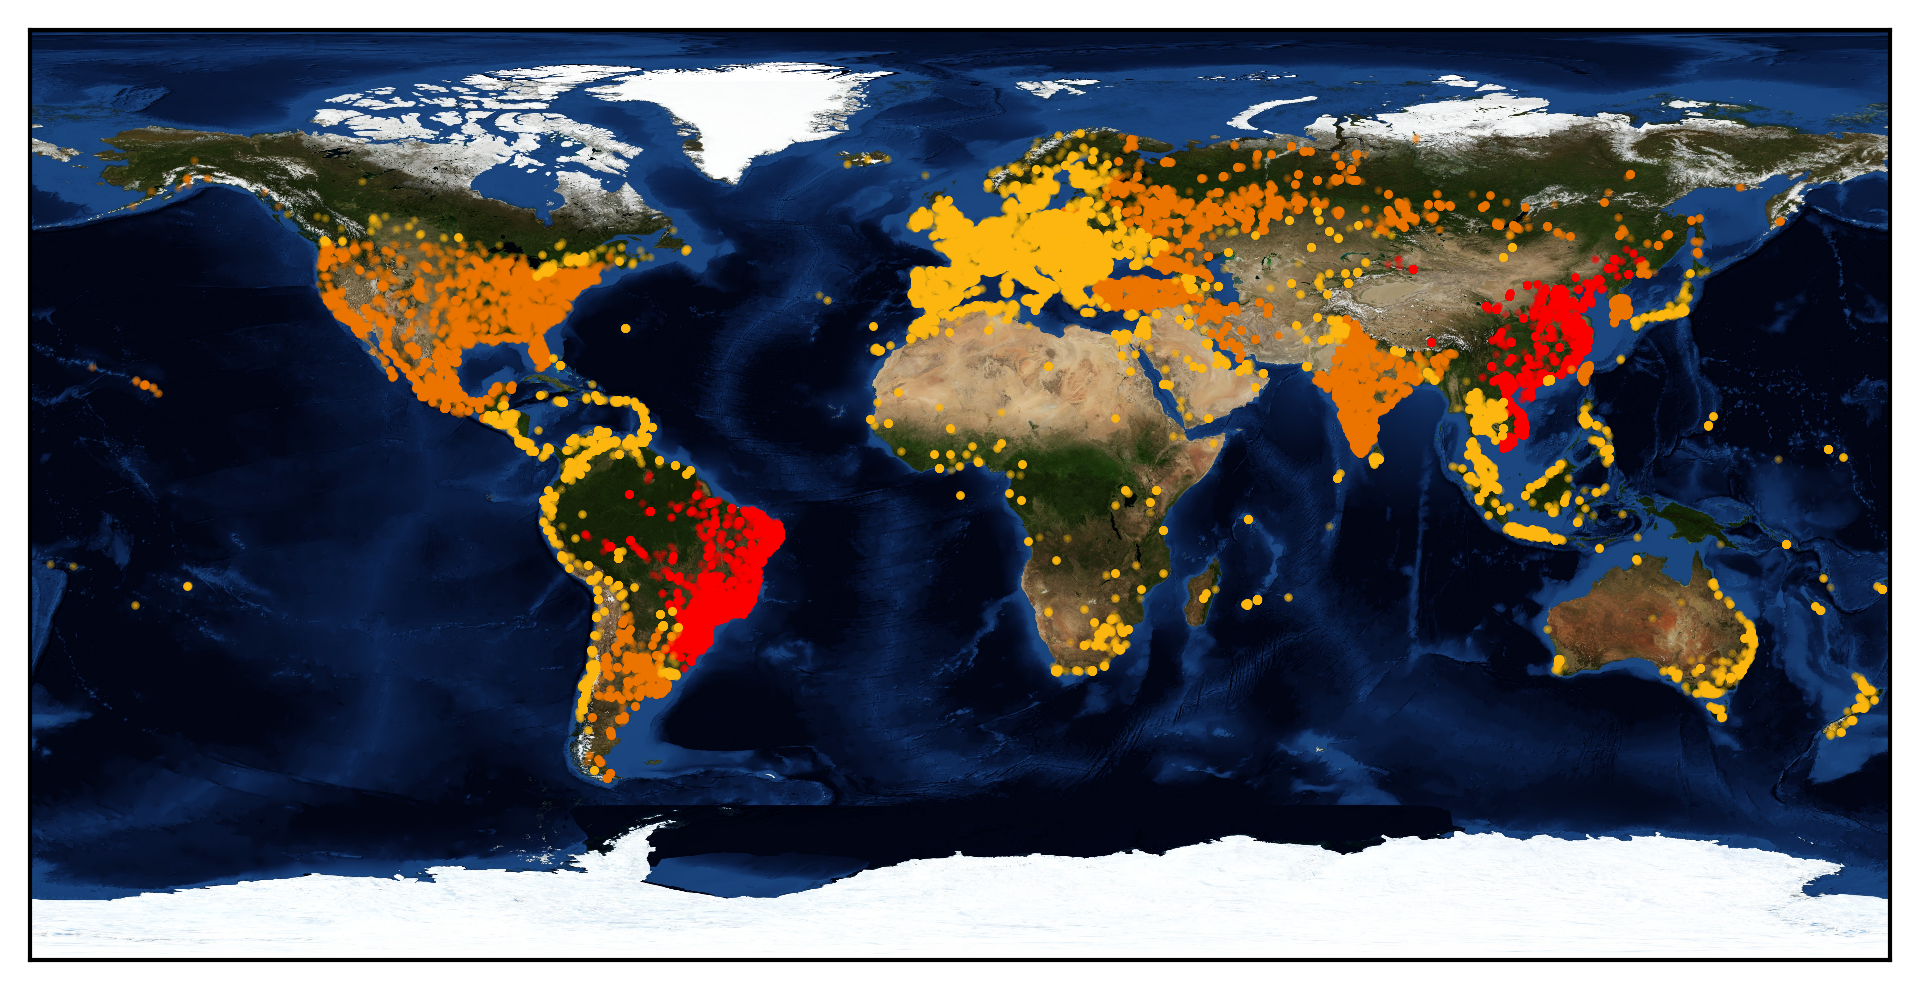
\includegraphics[width=14cm, height=8cm]{images/geographical_jan.png}
\caption{Geographic Distribution of Port Scan Source IP Addresses at First Configuration}
\end{figure}
\begin{figure}[p]
\centering
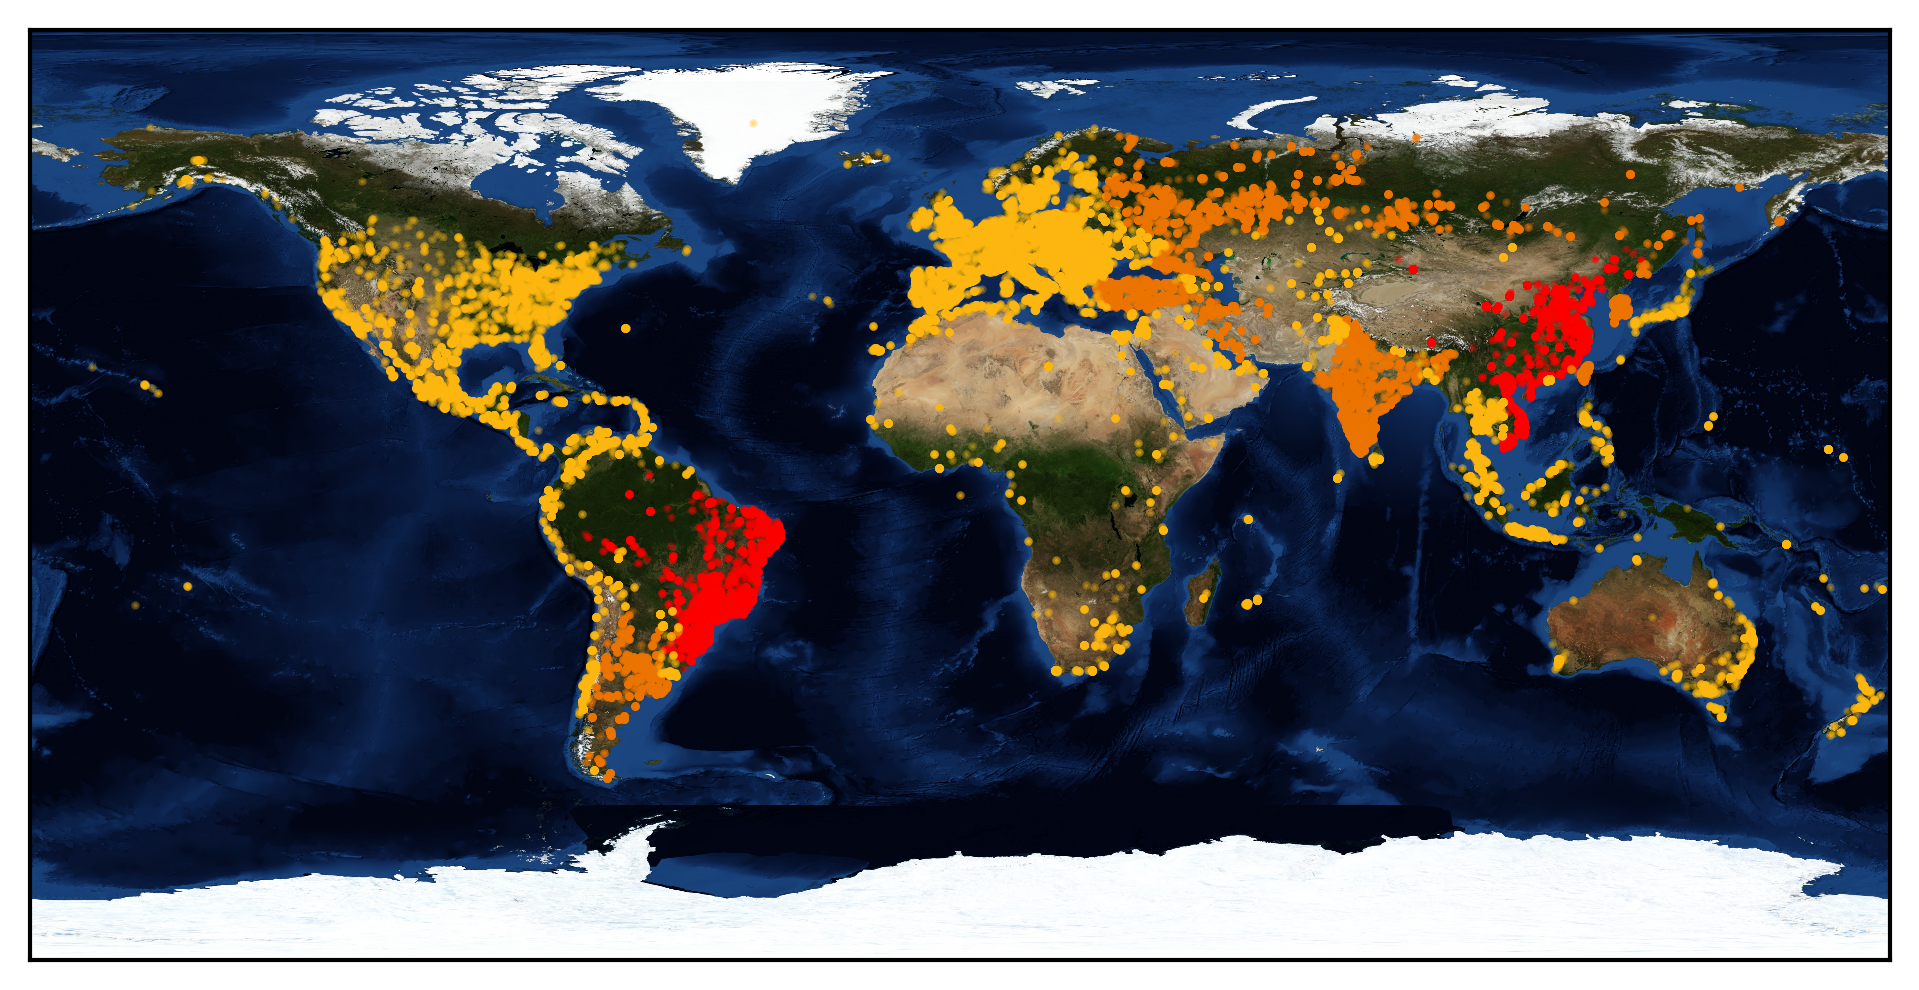
\includegraphics[width=14cm, height=8cm]{images/geographical_march.png}
\caption{Geographic Distribution of Port Scan Source IP Addresses at Second Configuration}
\end{figure}
\\\\ 
Figure 7.22 and Figure 7.23 show the geographical distribution of port scan source IP address at first and second configuration respectively.
These two heat maps show similar behavior in respect to the origin of port scans.
These maps show that port scans are a global phenomena and it originate from a multitude of locations across the world and seem to be correlated only with accessibility of the Internet. 

\chapter{Conclusion and Future Work}
\section{Conclusion}
Port scanning is great solution for researchers to study and evaluate new types of vulnerabilities, to track many risk mitigation activities.
On the other hand, it can be used by attackers to locate opened/vulnerable ports.
So we did a detailed study on how these port scans generally behave by analysing the captured packets using network telescope.
We analysed if port scans behavior will change if we combine network telescope with honeypot to capture the packets.
Moreover we also compared the behavior of TCP and UDP port scans with some common metrics.\\\\
We designed and implemented network forensic system to detect and study the behavior of port scanning attacks captured through first and second configuration of capturing system.
Several metrics such as horizontal and vertical scans, geographic distribution of scan sources, popular targeted services,relationship between traffic rate and the time of the day etc were used for better analysis and comparison of port scanning packets received through two separate network telescope configurations.
In addition to that, some of the above mentioned metrics were used for the comparison of TCP and UDP port scans.\\\\
We initially compared number of TCP and UDP port scans from both datasets.
We observed that TCP port scans are substantially greater in amount compared to UDP port scans during both first and second packet capturing period.
In horizontal scanning, we could not see any apparent difference in the behavior between port scans detected during first and second time period. 
However, number of horizontal scans keep reducing when number of
distinct destination IPs scanned by scan source increases in both datasets.
In vertical scanning, we could see an increase in vertical scanning activities in general in packets captured through second configuration compared to packets captured through first configuration.
Moreover, we noticed a large amount of small scans while only few number of large scans.\\\\
Another interesting metric for the comparison of port scans from two datasets is ports targeted in TCP and UDP scans.
It is evident from the analysis that, there is an increase in number of TCP and UDP ports scanned at second stage in respect to number of ports scanned at first stage.
In addition to that, we observed most actively scanned TCP and UDP ports during both time periods did not change much.
We also analysed relationship between traffic and time of the day
for TCP and UDP port scans from both datasets.
It is evident from the results we obtained that, TCP and UDP port scans do not show a correlation between traffic and time of the day.
However, TCP port scanning is a constant activity while UDP port scans are not very frequent as TCP port scanning activity.
Another property we analysed is how port scan source IP addresses are geographically distributed around the world.
We noticed that port scans are a global phenomena and it originate from a multitude of locations across the world and seem to be correlated only with accessibility of the Internet.
\section{Future Work}
While we shed light on the general behavior of port scanning activity , there stay a few open inquiries surrounding detection of port scans and protective mechanisms.
While we used two separate methods to correlate distributed scanners, it remains an open
research problem to detect and correlate distributed scanning events efficiently.
In this thesis work, we focused on scanning detection within the IPv4 address space.
Port scanning detection on IPv6 address space remains an open problem, as does analyzing existing IPv6 scanning behavior.
While, from the analysis, it was evident that majority of large port scans are originated from large hosting providers, it is in many cases hard to recognize the exact goal of the scanner beyond scanned protocol.
Follow-up work is important to decide the subsequent activities of these scanners.


%

%% Literature
%% \clearpage
\bibliographystyle{IEEEtran}
\bibliography{literature.bib}

%\cleardoublepage
%\phantomsection
%\addcontentsline{toc}{chapter}{Lists}
%\part*{Glossary and Lists}

\cleardoublepage
\phantomsection
\addcontentsline{toc}{section}{List of Tables}
\listoftables

\cleardoublepage
\phantomsection
\addcontentsline{toc}{section}{List of Figures}
\listoffigures

%\newpage
%\part{Appendices}
%\begin{appendices}
%\addcontentsline{toc}{section}{Obtaining quadratic form of a hyperbola from foci and length of semi-major axis}
%\input{chapters/converting_hyperbolas_eq.tex}
%\end{appendices}



\end{document}